%% abtex2-modelo-trabalho-academico.tex, v-1.9.2 laurocesar
%% Copyright 2012-2014 by abnTeX2 group at http://abntex2.googlecode.com/ 
%%
%% This work may be distributed and/or modified under the
%% conditions of the LaTeX Project Public License, either version 1.3
%% of this license or (at your option) any later version.
%% The latest version of this license is in
%%   http://www.latex-project.org/lppl.txt
%% and version 1.3 or later is part of all distributions of LaTeX
%% version 2005/12/01 or later.
%%
%% This work has the LPPL maintenance status `maintained'.
%% 
%% The Current Maintainer of this work is the abnTeX2 team, led
%% by Lauro César Araujo. Further information are available on 
%% http://abntex2.googlecode.com/
%%
%% This work consists of the files abntex2-modelo-trabalho-academico.tex,
%% abntex2-modelo-include-comandos and abntex2-modelo-references.bib
%%

% ------------------------------------------------------------------------
% ------------------------------------------------------------------------
% abnTeX2: Modelo de Trabalho Academico (tese de doutorado, dissertacao de
% mestrado e trabalhos monograficos em geral) em conformidade com 
% ABNT NBR 14724:2011: Informacao e documentacao - Trabalhos academicos -
% Apresentacao
% ------------------------------------------------------------------------
% ------------------------------------------------------------------------

\documentclass[
	% -- opções da classe memoir --
	12pt,				% tamanho da fonte
	openright,			% capítulos começam em pág ímpar (insere página vazia caso preciso)
	oneside,			% para impressão em verso e anverso. Oposto a oneside
	a4paper,			% tamanho do papel. 
	% -- opções da classe abntex2 --
	%chapter=TITLE,		% títulos de capítulos convertidos em letras maiúsculas
	%section=TITLE,		% títulos de seções convertidos em letras maiúsculas
	%subsection=TITLE,	% títulos de subseções convertidos em letras maiúsculas
	%subsubsection=TITLE,% títulos de subsubseções convertidos em letras maiúsculas
	% -- opções do pacote babel --
	english,			% idioma adicional para hifenização
	french,				% idioma adicional para hifenização
	spanish,			% idioma adicional para hifenização
	brazil				% o último idioma é o principal do documento
	]{abntex2}

% ---
% Pacotes básicos 
% ---
\usepackage{lmodern}			% Usa a fonte Latin Modern			
\usepackage[T1]{fontenc}		% Selecao de codigos de fonte.
\usepackage[utf8]{inputenc}		% Codificacao do documento (conversão automática dos acentos)
\usepackage{lastpage}			% Usado pela Ficha catalográfica
\usepackage{indentfirst}		% Indenta o primeiro parágrafo de cada seção.
\usepackage{color}				% Controle das cores
\usepackage{graphicx}			% Inclusão de gráficos
\usepackage{microtype} 			% para melhorias de justificação
% ---

%%CUSTOM
%Path relative to the main .tex file 
\graphicspath{ {./imagens/} }
%code highlight
\usepackage{minted}
\usepackage{booktabs}
\usepackage[final]{pdfpages}
\usepackage{afterpage}
\usepackage{hyperref}
\usepackage{dirtytalk}
\usepackage{array}
\usepackage{caption}
%%CUSTOM-FRED-END
		
% ---
% Pacotes adicionais, usados apenas no âmbito do Modelo Canônico do abnteX2
% ---
\usepackage{lipsum}				% para geração de dummy text
% ---

% ---
% Pacotes de citações
% ---
\usepackage[brazilian,hyperpageref]{backref}	 % Paginas com as citações na bibl
\usepackage[alf]{abntex2cite}	% Citações padrão ABNT

% --- 
% CONFIGURAÇÕES DE PACOTES
% --- 

% ---
% Configurações do pacote backref
% Usado sem a opção hyperpageref de backref
\renewcommand{\backrefpagesname}{Citado na(s) página(s):~}
% Texto padrão antes do número das páginas
\renewcommand{\backref}{}
% Define os textos da citação
\renewcommand*{\backrefalt}[4]{
	\ifcase #1 %
		Nenhuma citação no texto.%
	\or
		Citado na página #2.%
	\else
		Citado #1 vezes nas páginas #2.%
	\fi}%
% ---

% ---
% Informações de dados para CAPA e FOLHA DE ROSTO
% ---
\titulo{Desenvolvimento de Sistema para gerenciar e auxiliar na tomada de decisão envolvendo consumo de energia elétrica}
\autor{Rafael Ratacheski de Sousa Raulino}
\local{Goiânia}
\data{2019}
\orientador{Marcelo Stehling de Castro}
\instituicao{%
 Universidade Federal de Goiás - UFG
  \par
  Escola de Engenharia Elétrica, Mecânica e Computação
  \par
  Graduação em Engenharia de Computação}
\tipotrabalho{Projeto Final (Graduação)}
% O preambulo deve conter o tipo do trabalho, o objetivo, 
% o nome da instituição e a área de concentração 
\preambulo{Trabalho de Conclusão de Curso apresentado
ao Curso de Engenharia de Computação da Universidade
Federal de Goiás, como requisito parcial para obtenção
do grau de Engenheiro de Computação.}
% ---


% ---
% Configurações de aparência do PDF final

% alterando o aspecto da cor azul
\definecolor{blue}{RGB}{41,5,195}

% informações do PDF
\makeatletter
\hypersetup{
     	%pagebackref=true,
		pdftitle={\@title}, 
		pdfauthor={\@author},
    	pdfsubject={\imprimirpreambulo},
	    pdfcreator={LaTeX with abnTeX2},
		pdfkeywords={abnt}{latex}{abntex}{abntex2}{trabalho acadêmico}, 
		colorlinks=true,       		% false: boxed links; true: colored links
    	linkcolor=blue,          	% color of internal links
    	citecolor=blue,        		% color of links to bibliography
    	filecolor=magenta,      		% color of file links
		urlcolor=blue,
		bookmarksdepth=4
}
\makeatother
% --- 

% --- 
% Espaçamentos entre linhas e parágrafos 
% --- 

% O tamanho do parágrafo é dado por:
\setlength{\parindent}{1.3cm}

% Controle do espaçamento entre um parágrafo e outro:
\setlength{\parskip}{0.2cm}  % tente também \onelineskip

% ---
% compila o indice
% ---
\makeindex
% ---

% ----
% Início do documento
% ----
\begin{document}

% Retira espaço extra obsoleto entre as frases.
\frenchspacing 

% ----------------------------------------------------------
% ELEMENTOS PRÉ-TEXTUAIS
% ----------------------------------------------------------
% \pretextual

\imprimircapa
\imprimirfolhaderosto

%~~~~~~~~~~~~~~~~~~~~~~~~~~~~~~~~~~~~~~~~~~~~~~~~~~~~~~~~~~~~~~~~~~~~~
%   Arquivo     : fichaCatalografica.tex
%   Tipo        : TeX
%   Conteúdo    : Arquivo contendo a ficha catalográfica do Trabalho da EMC/UFG
%   Data        : 30 de abril de 2012
%   Copyright   : Marcelo Stehling de Castro
%   E-mail      : mcastro@ufg.br
%~~~~~~~~~~~~~~~~~~~~~~~~~~~~~~~~~~~~~~~~~~~~~~~~~~~~~~~~~~~~~~~~~~~~~

\begin{fichacatalografica}
	\sffamily
%	\vspace*{\fill}					% Posição vertical
	\begin{center}					% Minipage Centralizado
	\fbox{\begin{minipage}[c][8cm]{13.5cm}		% Largura
	\small
	\imprimirautor / \imprimirtitulo \par
	%Sobrenome, Nome do autor
	
	\imprimirtipotrabalho~--~\imprimirinstituicao,\imprimirlocal,\imprimirdata
	\newline
	\vspace{0.5cm}
	\hspace{0.5cm} \thelastpage p. : il. (algumas color.) ; 30 cm.
	\newline
    \hspace{0.5cm} \imprimirorientadorRotulo~\imprimirorientador
	\newline
		1. Desenvolvimento de Sistema \par
		2. Consumo Energético \par
		3. Monitoramento de rede energética \par
		I. {\imprimirinstituicao} \par
		II. \imprimirtitulo
	\end{minipage}}
	\end{center}
\end{fichacatalografica}
% ---
\vspace*{\fill}

\begin{minipage}{.9\textwidth}
        \textbf{CESSÃO DE DIREITOS}
	    \vspace{0.5cm}
	    
        AUTOR: Rafael Ratacheski de Sousa Raulino
        TÍTULO DA MONOGRAFIA: {\imprimirtitulo} 
        GRAU / ANO: Bacharel / {\imprimirdata} 
        
        O autor reserva outros direitos de publicação e nenhuma parte desta monografia pode ser reproduzida sem a autorização por escrito do autor.
        
	    \vspace{0.5cm}
        \begin{center}
            \begin{minipage}{.45\textwidth}
            \begin{center}
                {\imprimirautor}
            \end{center}
            \footnotesize{Endereço: Rua 16, Quadra C, Lote 4, Casa 1, Setor Morais, Goiânia - GO.} 
            \footnotesize{CEP: 74620-415.} 
            \footnotesize{Tel.: +55 62 99246-3302} 
            \footnotesize{E-mail: rafaelratacheski@gmail.com}
            \end{minipage}
        \end{center}
\end{minipage}

%~~~~~~~~~~~~~~~~~~~~~~~~~~~~~~~~~~~~~~~~~~~~~~~~~~~~~~~~~~~~~~~~~~~~~
%   Arquivo     : folhadeaprovacao.tex
%   Tipo        : TeX
%   Conteúdo    : Arquivo de referente a folha do Trabalho da EMC/UFG
%   Data        : 30 de abril de 2012
%   Copyright   : Marcelo Stehling de Castro
%   E-mail      : mcastro@ufg.br
%~~~~~~~~~~~~~~~~~~~~~~~~~~~~~~~~~~~~~~~~~~~~~~~~~~~~~~~~~~~~~~~~~~~~~

\begin{folhadeaprovacao}

  \begin{center}
    {\ABNTEXchapterfont\large\imprimirautor}

    \vspace*{\fill}\vspace*{\fill}
    \begin{center}
      \ABNTEXchapterfont\bfseries\Large\imprimirtitulo
    \end{center}
    \vspace*{\fill}
    
    \hspace{.45\textwidth}
    \begin{minipage}{.5\textwidth}
        \imprimirpreambulo
    \end{minipage}%
    \vspace*{\fill}
   \end{center}
        
   Trabalho aprovado. \imprimirlocal,       de           de 2018:

   \assinatura{\textbf{\imprimirorientador} \\ Orientador} 
   \assinatura{\textbf{Professor} \\ Convidado 1}
   \assinatura{\textbf{Professor} \\ Convidado 2}
   %\assinatura{\textbf{Professor} \\ Convidado 3}
   %\assinatura{\textbf{Professor} \\ Convidado 4}
      
   \begin{center}
    \vspace*{0.5cm}
    {\large\imprimirlocal}
    \par
    {\large\imprimirdata}
    \vspace*{1cm}
  \end{center}
  
\end{folhadeaprovacao}


\begin{dedicatoria}
   \vspace*{\fill}
   \centering
   \noindent
   \textit{ Este trabalho é dedicado às crianças adultas que,\\
   quando pequenas, sonharam em se tornar cientistas.} \vspace*{\fill}
\end{dedicatoria}

\begin{agradecimentos}
Os agradecimentos principais são direcionados à Gerald Weber, Miguel Frasson,
Leslie H. Watter, Bruno Parente Lima, Flávio de Vasconcellos Corrêa, Otavio Real
Salvador, Renato Machnievscz\footnote{Os nomes dos integrantes do primeiro
projeto abn\TeX\ foram extraídos de
\url{http://codigolivre.org.br/projects/abntex/}} e todos aqueles que
contribuíram para que a produção de trabalhos acadêmicos conforme
as normas ABNT com \LaTeX\ fosse possível.

Agradecimentos especiais são direcionados ao Centro de Pesquisa em Arquitetura
da Informação\footnote{\url{http://www.cpai.unb.br/}} da Universidade de
Brasília (CPAI), ao grupo de usuários
\emph{latex-br}\footnote{\url{http://groups.google.com/group/latex-br}} e aos
novos voluntários do grupo
\emph{\abnTeX}\footnote{\url{http://groups.google.com/group/abntex2} e
\url{http://abntex2.googlecode.com/}}~que contribuíram e que ainda
contribuirão para a evolução do \abnTeX.

\end{agradecimentos}

\begin{epigrafe}
    \vspace*{\fill}
	\begin{flushright}
		\textit{``Não vos amoldeis às estruturas deste mundo, \\
		mas transformai-vos pela renovação da mente, \\
		a fim de distinguir qual é a vontade de Deus: \\
		o que é bom, o que Lhe é agradável, o que é perfeito.\\
		(Bíblia Sagrada, Romanos 12, 2)}
	\end{flushright}
\end{epigrafe}



% ---
% RESUMOS
% ---

% resumo em português
\setlength{\absparsep}{18pt} % ajusta o espaçamento dos parágrafos do resumo
\begin{resumo}
 Nos últimos anos com o intenso desenvolvimento de dispositivos eletrônicos para facilitar nosso dia a dia, o consumo de energia elétrica só tem aumentado, e juntamente a esse aumento cresceu-se também o impacto ambiental e econômico causado por esse consumo. Sendo assim a preocupação em se criar medidas para o entendimento e o controle dos impactos é cada dia mais presente. Propõe-se com este trabalho, desenvolvimento de um sistema, para fazer o monitoramento e auxiliar no controle da rede energética da Universidade Federal de Goiás disponibilizando uma interface para apreciação dos dados coletados pelos sistemas de monitoramento da rede energética, fazer o cadastramento em uma base do seu acervo de materiais geradores e transportadores de energia, juntamente com a possibilidade de inserção de dados históricos do consumo através de envio de faturas das unidades consumidoras da Universidade, alimentando o banco de dados do sistema com os dados oficiais da concessionária de energia de faturamento dos meses passados. 

 \textbf{Palavras-chaves}: consumo energético. banco de dados. monitoramento de rede energética. sistema de monitoramento.
\end{resumo}

% resumo em inglês
\begin{resumo}[Abstract]
 \begin{otherlanguage*}{english}
   In recent years with the intense development of electronic devices to facilitate our day to day, electricity consumption has only increased, and along with this increase has also grown the environmental and economic impact caused by such consumption. Therefore, the concern to create measures for the understanding and control of impacts is increasingly present. It is proposed, with this work, the development of a system to monitor and assist in the control of the energy network of the Federal University of Goiás, providing an interface for appreciation of the data collected by the energy grid monitoring systems, of its collection of generating materials and energy carriers, together with the possibility of inserting historical consumption data by sending invoices from the University's consuming units, feeding the system database with the official data of the billing energy utility of past months.

   \vspace{\onelineskip}
 
   \noindent 
   \textbf{Key-words}: energy consumption. database. energy network monitoring. monitoring system.
 \end{otherlanguage*}
\end{resumo}


% ---
% inserir lista de ilustrações
% ---
\pdfbookmark[0]{\listfigurename}{lof}
\listoffigures*
\cleardoublepage
% ---

% ---
% inserir lista de tabelas
% ---
\pdfbookmark[0]{\listtablename}{lot}
\listoftables*
\cleardoublepage
% ---

\begin{siglas}
  \item[SGBD] Sistema Gerenciador de Banco de Dados
  \item[SIDE] Sistema Interpretador de Dados Energéticos
  \item[PDF] Portable Document Format
  \item[DB] \textit{Database} (Banco de Dados)
  \item[UFER] Unidade de Faturamento de Energia Reativa
  \item[DMCR] Demanda Máxima Corrigida
  
\end{siglas}

\begin{simbolos}
  \item[$ \Gamma $] Letra grega Gama
  \item[$ \Lambda $] Lambda
  \item[$ \zeta $] Letra grega minúscula zeta
  \item[$ \in $] Pertence
\end{simbolos}

\renewcommand{\listingscaption}{Algoritmo}
\renewcommand{\listoflistingscaption}{Lista de Códigos Fonte}
\listoflistings
\cleardoublepage


% ---
% inserir o sumario
% ---
\pdfbookmark[0]{\contentsname}{toc}
{
  \hypersetup{linkcolor=black}
  \tableofcontents*
}
\cleardoublepage
% ---

% ----------------------------------------------------------
% PARTE
% ----------------------------------------------------------
\part{Introdução}
% ----------------------------------------------------------

% ---

% ----------------------------------------------------------
% ELEMENTOS TEXTUAIS
% ----------------------------------------------------------
\textual

\chapter[Introdução ao Problema]{Introdução ao Problema}

Nesta introdução serão apresentados os objetivos do trabalho, a definição de alguns conceitos que se fazem necessários para que este se situe e para que a motivação e desafios do mesmo sejam esclarecidos e, por fim, a estrutura da monografia.

\section{Objetivos}

Os objetivos principais deste trabalho são:

\begin{itemize}
    \item desenvolver um sistema para comunicação com os medidores de energia elétrica instalados na universidade;
    \item desenvolver um modelo de dados para armazenamento dos dados coletados por esses medidores, bem como os dados da própria concessionária de energia;
    \item desenvolver um sistema para leitura, interpretação e armazenamento dos dados contidos nas faturas energéticas geradas pela concessionária;
    \item implantar o sistema e disponibilizá-lo para o uso da instituição;
\end{itemize}

\section{Motivação}

A motivação desse trabalho surgiu no desenvolvimento inicial de um projeto durante estágio na instituição, onde o escopo inicial do sistema de interpretação dos dados das faturas energéticas foi definido, e onde posteriormente foi inserido a parte de comunicação com os medidores e a criação de uma interface para apreciação dos dados durante o desenvolvimento do \textbf{Projeto de Final de Curso 1} do mesmo autor descrito e disponível no apêndice \ref{a:PFC1}.

\section{Conceitos}

A seguir, serão abordados alguns dos conceitos de alto nível utilizados ao longo do trabalho, estes conceitos possibilitarão um entendimento inicial das técnicas escolhidas para a solução do problema inicial, bem como possibilitarão uma aproximação maior do leitor ao tema.

\newpage
\subsection{Protocolo Modbus}

O protocolo Modbus é uma estrutura de mensagem aberta desenvolvida pela Modicon na década de 70, utilizada para comunicação entre  dispositivos mestre-escravo / cliente-servidor. \cite{modicon1996}

Após a compra da Modicon pela Schneider os direitos sobre o protocolo foram liberados pela Organização Modbus. Muitos equipamentos industriais utilizam o Modbus como protocolo de comunicação, e graças às suas características, este protocolo também tem sido utilizado em uma vasta gama de aplicações como:

\begin{itemize}
\item  Instrumentos e equipamentos de laboratório;
\item  Automação residencial;
\item  Automação de navios;
\end{itemize}

\subsection{Desenvolvimento Ágil}

A partir de 1990 as definições desenvolvimento de software evoluíram como parte de uma reação contra métodos desgastantes de desenvolvimento, caracterizados por uma densa regulamentação. 

O processo originou-se da visão de que o modelo em cascata era burocrático e lento, uma forma contrária com a qual engenheiros de software realizavam seus trabalhos.
Inicialmente, foram desenvolvidas técnicas para para agilizar o desenvolvimento e a esse conjunto de técnicas foi dado o nome de métodos leves. 

Em 2001, membros da comunidade se reuniram em \textit{Snowbird} e publicaram um manifesto para reunir os princípios e práticas desta metodologia de desenvolvimento, dando o nome de Manifesto Ágil \cite{beck2001manifesto}. Posteriormente, formou-se a \textit{Agile Alliance}, uma organização sem fins lucrativos que ajuda na divulgação do desenvolvimento ágil.

\newpage
\subsection{Banco de Dados}

\citeonline{korth1994} define um banco de dados como sendo \say{uma coleção de dados inter-relacionados, representando informações sobre um domínio específico}, ou seja, quando houver a possibilidade de se agrupar dados que se relacionam e fazem parte de um mesmo universo de um assunto, pode-se dizer que tem-se um banco de dados.

Já um sistema de gerenciamento de banco de dados (SGBD) é um \textit{software} que possibilita o usuário de fazer a manipulação e visualização, das informações gravadas no banco de dados. O SGBD adotado para o desenvolvimento deste projeto foi o PostgreSQL.

Fazendo o uso de um SGBD para acessar as informações do banco de dados, tem-se então o conceito de sistema de banco de dados como o conjunto de quatro componentes básicos: dados, hardware, software e usuários. \cite{date2004} conceituou que \say{sistema de bancos de dados pode ser considerado como uma sala de arquivos eletrônica}.


\section{Estrutura do trabalho}

Tendo como objetivo uma apresentação do cenário energético e econômico brasileiro atual, este trabalho faz um levantamento de dados de pesquisa e valores de consumos da instituição analisada no capítulo \ref{c:contextualizando_o_cenario_energetico_brasileiro}.

Logo após, um aprofundamento nos processos gerais de comunicação dos medidores através do protocolo Modbus e no processo de desenvolvimento de um sistema web, é feito nos capítulos \ref{c:a_comunicacao_modbus} e \ref{c:o_desenvolvimento_de_aplicacoes_web}.

Tendo a base conceitual das etapas, técnicas e problemas bem definida e contextualizada, a infraestrutura que fornecerá os dados para esse sistema e seus devidos meios de comunicação serão expostos no capítulo \ref{c:infraestrutura_da_rede_de_medidores}.
A exposição da modelagem inicial do banco que fará o armazenamento dos medidores e suas medições, das unidades consumidoras e suas devidas faturas energéticas, bem como todas as tabelas auxiliares para o funcionamento do sistema estarão declarados no capítulo \ref{c:estrutura_de_banco_de_dados}.

Expostos os modelos de como estarão distribuídas e armazenadas as informações serão explanados os subsistemas que irão compor a estrutura do Sistema Interpretador de Dados Energéticos (SIDE), sendo o sistema sincronizador de dados de medição descrito no capítulo \ref{c:sistema_sincronizador_de_dados}, o sistema interpretador de faturas descrito no capítulo \ref{c:sistema_interpretador_de_faturas}, e o sistema de interface com o usuário que fará a utilização de todos os outros subsistemas apresentado no capítulo \ref{c:interface_de_usuario}.

Por fim, os resultados encontrados e confirmados ao longo do projeto são dispostos nos capítulos \ref{c:obtencao_dos_dados_dos_sensores}, \ref{c:obtencao_dos_dados_das_faturas} e \ref{c:resultado_da_interface_do_usuario}, as conclusões deste apresentadas no capítulo \ref{c:conclusoes} e uma análise das possibilidades e trabalhos futuros na área no capítulo \ref{c:trabalhos_futuros}.



% ----------------------------------------------------------
% PARTE
% ----------------------------------------------------------
\part{Referenciais teóricos}
% ----------------------------------------------------------

\chapter{Contextualizando o Cenário Energético Brasileiro}
\label{c:contextualizando_o_cenario_energetico_brasileiro}
% ---

Como mostrado anteriormente, o projeto a ser desenvolvido está totalmente inserido
na abordagem de energia e consumo energético. Por isso é muito importante apresentar de maneira resumida o contexto histórico que estimula cada vez mais o estudo de soluções para possibilitar um consumo mais consciente dos recursos energéticos. 

% ---
\section{Aumento do Consumo de Energia}
% ---
O consumo de energia é um dos principais índices de
desenvolvimento econômico e qualidade de vida
da sociedade. Através dele podemos analisar tanto o ritmo de atividade
do comércio e das indústrias, quanto a
disponibilidade da população em adquirir bens e serviços
mais avançados tecnologicamente, como eletrônicos, automóveis, eletrodomésticos e serviços que necessitam do consumo energético para seu funcionamento.

Além do desenvolvimento econômico, outro fator ao qual o consumo de energia está diretamente relacionado é o crescimento populacional – indicador obtido pelo cálculo diferença entre as taxas de natalidade e mortalidade associado à medição de fluxos migratórios. No Brasil, no período de 2000 a 2005, o crescimento populacional teve uma tendência de queda relativa, registrando variação média anual de 1,46\%, segundo relata o estudo Análise Retrospectiva constante do Plano Nacional de Energia 2030, produzido pela Empresa de Pesquisa Energética.

Ainda assim, a tendência do consumo de energia no período foi de crescimento: 13,93\%, mostrando que mesmo que com uma queda do crescimento populacional a influência do crescimento econômico do cenário analisado se mostrou como mais influente sobre o consumo energético populacional. O Produto Interno Bruto do país, no mesmo período, registrou um
crescimento acumulado de 14,72\%, conforme dados do Ipea.

Analisando um cenário mais recente pode-se observar também aumento no consumo de energia elétrica no país, que totalizou 463.948 gigawatts-hora (GWh) em 2017, correspondendo a um crescimento de 0,8\%, segundo levantamento da Empresa de Pesquisa Energética (EPE). Somente em dezembro, o consumo foi de 39.288 GWh, alta de 1,7\% em relação ao verificado no mesmo período do ano anterior. \cite{atlasenergetico}


O consumo no mercado cativo (atendido pelas distribuidoras) teve queda de 5,6\% em 2017 e de 3\% em dezembro, influenciada pela migração de consumidores para o mercado livre, que cresceu 18,4\% e 13,7\%, respectivamente.

Dentre as classes de consumo, destaque para o segmento industrial, que cresceu 1,3\% no ano de 2017, alcançando 165.883 GWh, após duas quedas consecutivas nos anos anteriores, reflexo da melhora no cenário econômico, o que reforça a dependência direta entre o consumo e a economia.

% ---
\section{Utilização de Fontes Renováveis}
% ---

As energias renováveis se tornam cada vez mais atraentes como alternativa de micro geração distribuída uma vez que houve redução do preço de cédulas fotovoltaicas e aero geradores, já que atualmente aliado ao poder de compra do consumidor está o alto valor de conta de energia elétrica pago pelo brasileiro, considerada uma das contas mais elevadas no mundo. \cite{barbosa2013geraccao}

Fazendo uma análise inicial, as fontes renováveis, aparentemente, possuem um custo final mais elevado do que o sistema convencional centralizado de fornecimento energético. Entretanto o processo como um todo de produção da energia promove uma consequente redução
em seu valor total quando todos os processos necessários são contabilizados.

Os recursos fósseis necessitam de extração, transporte para as refinarias onde são preparados para a queima e, após a geração de eletricidade, esta deve ser transmitida através de linhas de alta tensão para o consumidor, enquanto que os resíduos devem ser eliminados. A utilização de máquinas rotativas, tais como turbina e gerador, necessitam de uma extensa rotina de manutenção , devido ao desgaste natural das peças móveis, além de gerar poluição sonora durante o seu funcionamento. Por outro lado, a energia solar não necessita de um pesado e caro processo de extração, não demanda refinamento e nem transporte para o local da consumo, devido o mesmo ser o qual é próximo ao local de geração, evitando assim os custos com a transmissão em alta tensão. Utiliza células solares, responsáveis pela geração de energia, e um inversor para transformar a tensão gerada em corrente contínua para os valores nominais dos aparelhos de consumo em corrente alternada. Este processo é mais simples, sem emissão de gases poluentes ou ruídos e com uma pequena dependência de manutenções periódicas.\cite{galdino2000contexto}

Os custos envolvendo todas estas etapas necessárias para a geração de
energia devem ser computados no momento em que se compara a energia solar
com as outras fontes. Devido à sua simplicidade, esta forma renovável de obter
eletricidade possui vantagens econômicas. 
\chapter{A Comunicação \textit{Modbus}}
\label{c:a_comunicacao_modbus}
% ---
\section{O protocolo \textit{Modbus}}

O \textit{Modbus} é um protocolo amplamente utilizado no setor de automação industrial, principalmente por sua simplicidade e facilidade de implementação. Este protocolo permite que seja usada uma mesma linguagem de comunicação em diversos padrões de meio físico, variando a velocidade de comunicação, quantidade de dispositivos suportados na rede bem como o comprimento máximo da mesma, fazendo assim com que cada tipo de estrutura física seja adequada à um cenário de projeto, justificando com isso a sua ampla utilização.

Os padrões de meio físico definem o modo de comunicação através do qual os dados serão transmitidos entre o mestre e seus escravos. O protocolo pode ser utilizado por uma aplicação por um meio serial ou através de conexões TCP (\textit{Ethernet}), tendo por exemplo os padrões RS-232,RS-4222 e RS-485 para a comunicação serial e o modbus TCP para a comunicação através de endereços IP para cada dispositivo \cite{dutertre2007formal}.

O padrão RS-232 (Recommended Standard 232) ou EIA-232 (Electronic Industries Alliance 232) é utilizado apenas quando se possui apenas dois dispositivos na rede, formando a chamada comunicação ponto a ponto,  onde no protocolo \textit{Modbus} representa o mestre e o escravo. Este padrão alcança velocidades em uma média de 115 Kbps, podendo ultrapassar este valor em um pequeno percentual, dependendo da qualidade estrutural da rede. A distância máxima entre o escravo e o mestre da rede é de aproximadamente 30 metros.

O padrão RS-485 (Recommended Standard 485) ou EIA-485 (Electronic Industries Alliance 485) é um dos padrões mais utilizados industrialmente, dentre os outros com comunicação serial. Uma das principais vantagens em relação ao RS-232 é que a comunicação mestre escravo não fica limitada a apenas dois dispositivos, podendo estabelecer uma comunicação de até 32 dispositivos por barramento na rede. Além disso a sua velocidade de conexão é bem superior aos 115 Kbps descritos no parágrafo anterior, podendo chegar à 50Mbps, dependo do comprimento da rede, sendo que quanto maior for, menor será a velocidade de comunicação sendo que nesse caso o alcance máximo da rede é por volta de 1200 metros.


Já o protocolo TCP, como o próprio nome sugere, utiliza TCP como camada de comunicação, porém tentando manter uma compatibilidade com o protocolo serial Modbus. Para possibilitar a diferenciação de cada escravo é atribuído um endereço IP para o dispositivo através do qual o mesmo será identificado na rede, além disso o protocolo \textit{Modbus} TCP utiliza por padrão um número de porta IP específico (502) para a comunicação. O Modbus TCP possui uma vantagem econômica devido à maior facilidade de implantação por conta da ampla disponibilidade de redes compatíveis com a comunicação TCP, porém esta alta disponibilidade traz consigo uma preocupação maior em relação à segurança dos dados transmitidos na rede. 


\section{Formato de uma mensagem \textit{Modbus}}

A estrutura de uma mensagem transmitida com base 
no protocolo \textit{Modbus} RTU é definida 
na imagem a seguir, porém podemos utilizar a mesma 
como base para o modelo ASCII 
diferenciando-se por um caractere inicial ":" (ASCII 0x3Ah) 
e um CRLF (\textit{Carriage Return and Line Feed}) 
representado em ASCII por 0x0Dh + 0x0Ah ao final da mensagem:
\newline

\begin{figure}[h]
\caption{Estrutura da Mensagem \textit{Modbus}}
\centering
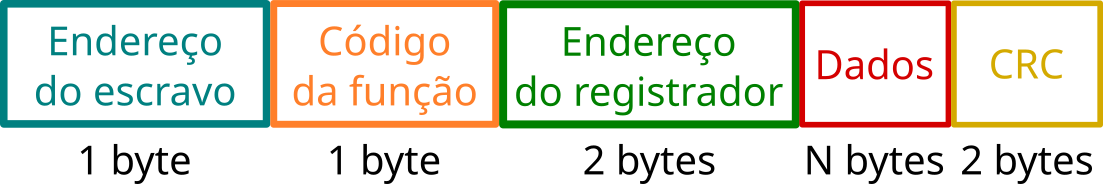
\includegraphics[width=1.0\textwidth,height=1.0\textheight,keepaspectratio]{imagens/mensagem-modbus.png}
\caption*{Fonte: Próprio Autor}
\end{figure}

\subsection{Endereçamento}

No caso da comunicação serial a mensagem conterá inicialmente 1 byte com o endereçamento do dispositivo de destino da mensagem, podem ir de 1 a 256. Já para a comunicação TCP o início da mensagem conterá um cabeçalho que basicamente é composto pelo endereçamento IP do dispositivo de destino da mensagem.

\subsection{Função}

Neste campo de 1 byte o dispositivo mestre indicará qual o tipo de serviço ou função que será solicitada ao escravo. No protocolo \textit{Modbus}, cada função é utilizada para acessar um tipo específico de dado. Algumas dessas funções estão descritas na tabela abaixo para efeito de exemplificação.


\begin{table}[H]
\centering
\caption{Lista de Algumas Funções do Protocolo Modbus}
\label{tab:tabela_funcoes_modbus}
\begin{tabular}{| l | m{11cm} |}
\hline
\textbf{Código da Função} & \textbf{Descrição} \\ [10pt]
\hline
0x01 & Leitura de bloco de bits do tipo coil (saída discreta) \\ 
\hline
0x02 & Leitura de bloco de bits do tipo entradas discretas \\ 
\hline
0x03 & Leitura de um número variável de registros retentivos (saídas analógicas ou memórias) \\ 
\hline
0x04 & Leitura de um número variável de registros de entrada (entradas analógicas)\\ 
\hline
0x05 & Escrita em um único bit do tipo coil (saída discreta) \\ 
\hline
0x06 & Escrita em um único registrador (altera o estado de uma saída analógica)\\ 
\hline
0x07 & Leitura do conteúdo de 8 estados de exceção (registro de erros) \\ 
\hline
0x08 & Execução de uma série de testes para verificação da comunicação e erros internos\\ 
\hline
\end{tabular}
\end{table}

\subsection{Dados}

Este campo possui um tamanho em bytes variável dependendo do conteúdo de retorno da mensagem solicitada pelo mestre através do código da função passada ou da informação que será registrada no escravo, sendo que esta mensagem será inserida no corpo da mensagem pelo mestre.

\subsection{CRC}

Para os protocolos com comunicação serial, ao final da mensagem existirão 2 bytes contendo uma mensagem de verificação de erros na transmissão da mesma, preenchidos por um algoritmo de CRC (\textit{Cyclic Redundancy Check}). Essa mensagem garantirá a consistência do envio completo da mensagem.
Já para o protocolo de comunicação TCP, os bytes finais de verificação de erro já não se fazem necessários.



\chapter{O Desenvolvimento de Aplicações \textit{Web}}
\label{c:o_desenvolvimento_de_aplicacoes_web}
% ---

Neste capítulo, serão apresentadas as etapas envolvidas no desenvolvimento da aplicação deste trabalho, que vaõ desde o levantamento de requisitos, criação de um versionamento e utilização de conceitos de engenharia de \textit{software}.

\section{Levantamento de Requisitos}

O levantamento de requisitos é uma importante etapa para a concepção de um projeto no âmbito da engenharia de requisitos, onde a pessoa responsável pela análise deve fazer o uso de todas informações disponíveis que definirão os requisitos para poder identificar as funcionalidades que o sistema deverá ter \cite{wazlawick2013engenharia}.

\cite{bezerra2016principios} define para o levantamento de requisitos os seguintes meios de obtenção 
\begin{itemize}
    \item questionários, tendo por objetivo a descoberta de problemas a serem abordados, identificar os principais procedimentos e definir a expectativa dos entrevistados têm a respeito do produto;
    \item entrevistas, que consistem em diálogos direcionadas à um fornecedor de requisitos no formato “pergunta-resposta” com um propósito específico tendo os mesmos objetivos dos questionários;
    \item observação, que consiste em fazer uma análise externa do comportamento e o ambiente dos indivíduos de vários níveis organizacionais, capturando as necessidades, modo de trabalho e as deficiências de cada atividade relacionada ao projeto; 
    \item entre outros.
\end{itemize}

O processo de levantar os requisitos de um projeto é um tanto quanto complexa, pois um escopo mal definido ou um mau entendimento dos usuários quanto às capacidades e limitações do sistema computacional  podem se tornar um grande problema para o projeto como um todo, além da própria volatilidade dos requisitos, que mudam ao longo da execução do mesmo \cite{pressman2016engenharia}.

Em casos onde são utilizados diagramas de atividades para modelar os principais processos aos quais a aplicação deve abranger, o levantamento de requisitos deve identificar quais as funções são necessárias para realizar as atividades destes processos corretamente \cite{wazlawick2013engenharia}. Por este motivo, uma boa prática é que a primeira atividade do levantamento de requisitos seja a modelagem do negócio,através da construção de diagramas de atividades que descrevam detalhadamente os processos do negócio.

\section{Versionamento}

Versionamento ou controle de versão é o uso de ferramentas para realizar o gerenciamento de alterações ou diferentes versões no desenvolvimento de um determinado documento, projeto ou aplicação.

Os sistemas de controle de versão, comumente utilizados no desenvolvimento de \textit{software}, são ferramentas com o objetivo de gerenciar as inúmeras alterações nos documentos produzidos ao longo do processo de desenvolvimento.

De acordo com \cite{murta2006gerencia}, do ponto de vista do desenvolvimento, o gerenciamento de software é dividido em três sistemas principais, que são: controle de modificações, controle de versões e gerenciamento de construção.

Segundo \cite{mason2006pragmatic}, um sistema de controle de versão é basicamente um local para armazenamento de artefatos gerados durante o desenvolvimento de um sistema. Atuando como uma espécie de controle do tempo para a equipe de desenvolvimento, as ferramentas de controle de versão permitem a navegação por múltiplos arquivos de múltiplos autores a qualquer versão anterior.

Segundo \citeonline{araujo2019} as vantagens encontradas nos sistemas que utilizam mecanismos de controle de versão são: 
 \begin{itemize}
     \item Controle de histórico: Possibilita o usuário fazer a análise e comparação de versões anteriores do projeto podendo exportá-las e executá-las, podendo inclusive desfazer alterações voltando o documento ao estado em que se identificava nas versões anteriores.
     \item Suporte a colaboração: Possibilita a identificação de alteração de determinado documento,permitindo ao usuário interessado em alterar o mesmo documento, optar por aguardar a liberação do usuário que está trabalhando atualmente no documento, ou trabalhar de forma paralela, e posteriormente os usuários podem efetuar o \textit{merge} (mesclar informações de dois ou mais documentos a fim de gerar um só).
    \item Suporte a marcação e resgate de versões estáveis: Alguns sistemas de controle de versão possuem propriedades que identificam versões estáveis, possibilitando através do histórico, selecionar uma versão estável para exportar e utilizar.
    \item Ramificação de projeto: Possibilita o trabalho por equipes diferentes em um mesmo produto, onde esses ramos posteriormente podem ser unidos ao projeto principal através de uma solicitação ao gerente do sistema de versionamento.
 \end{itemize}

\newpage

Nos documentos de especificação de software o emprego desses
mecanismos de gerenciamento de versões é essencial. Os requisitos mudam
constantemente devido a variados motivos, podendo eles ser desde ao fato de os problemas aos quais se refere um requisito não foram inteiramente definidos, desde uma evolução no entendimento dos desenvolvedores acerca do problema, passando por melhorias em sistemas antigos ou automatização de algum processo manual. Além disso, regras e ambiente técnico também são fatores para uma atualização nos requisitos de software. Dessa forma, requisitos podem ser atualizados, incluídos ou removidos.

Certo de que estes documentos representam determinada funcionalidade ou
propriedade de um sistema, e impõe grandes responsabilidades de quem for alterá-los, fica necessário o rastreamento das mudanças, por conta disso, opções de acesso a leitura de versões anteriores, para o usuário poder comparar versões, são peças fundamentais nos gerenciadores de requisitos de software. 

\section{Engenharia de Software}

De acordo com \cite{pressman2016engenharia}, a engenharia de software pode ser definida como \say{aplicação de uma abordagem sistemática, disciplinada e quantificável, para desenvolvimento, operação e manutenção do software, isto é a aplicação da engenharia ao software}.

A evolução da complexidade no processo de produção de um software, devido à novos dispositivos, tecnologias e a melhoria nas comunicações e redes trouxe novos problemas para engenheiros e desenvolvedores. Devido estes e outros fatores, houve a necessidade de representar o processo em modelos que tentam se adaptar a essa nova realidade.

\subsection{Modelos de Processo}

Um modelo de processo de software, de acordo com \cite{sommerville2011software}, é uma representação abstrata de um processo de software. Cada modelo de processo representa um processo a partir de uma perspectiva particular, de maneira que proporciona apenas
informações parciais sobre o processo. O modelo de processo abordado neste sistema será um modelo baseado em métodos ágeis com adaptações devido a ausência de equipe, oferecendo agilidade e uma metodologia indispensáveis aos projetos atuais, de acordo com \cite{beck2001manifesto}.

\subsection{Métodos Ágeis}

Embora os métodos ágeis estejam sendo aplicados a muito tempo, recentemente vem se tornando cada vez mais popular no Brasil devido ao fato de ser uma abordagem simplificada. Entretanto essa simplicidade e aceleração requerem disciplina e organização.

Em 2001, um grupo de 17 autores e representantes de diversas técnicas e metodologias se reuniram com o objetivo de estabelecer um padrão de desenvolvimento de projeto com as técnicas e metodologias existentes na época. O resultado final dessa reunião foi o Manifesto para o Desenvolvimento Ágil de Software \cite{beck2001manifesto}, que definiu um \textit{framework} comum para processos ágeis, trazendo novas ideias e sugestões para a melhoria de processos, técnicas e métodos de desenvolvimento e gestão de projetos de forma ágil.

De acordo com \cite{pressman2016engenharia}, a utilização de métodos ágeis pode trazer benefícios como: 
\begin{itemize}
    \item maior satisfação dos clientes;
    \item melhoria na comunicação e aumento na colaboração entre envolvidos nos projetos;
    \item melhoria na qualidade do produto;
    \item menores custos de produção;
\end{itemize} 

\subsection{Uso de Framework para Desenvolvimento de Aplicações}

Várias definições sobre framework são descritas na literatura, mas segundo \cite{gammapadroes} \say{um framework é um conjunto de classes que cooperam entre si provendo assim um projeto reutiliável para um domínio específico de classes de sistema}

Um \textit{framework} é uma estrutura de suporte definida através da qual outro projeto de software pode ser estruturado e desenvolvido. Um
\textit{framework} pode incluir programas de suporte, bibliotecas, modelagens de dados, linguagens de script e outros softwares para ajudar a desenvolver e juntar diferentes componentes de um novo projeto. 

Utilizando \textit{frameworks} tem-se como principal vantagem a redução de custos, devido ao fato de já existir uma estrutura definida, podendo assim a etapa de desenvolvimento concentrar-se apenas em implementar as regras específicas do negócio em que o sistema deve atuar. 

Um \textit{framework} ainda proporciona a reutilização de códigos e a fatoração de problemas em aspectos comuns a várias aplicações, permitindo a criação de sistemas com códigos menos frágeis e menos suscetíveis à defeitos. 

% ----------------------------------------------------------
% PARTE
% ----------------------------------------------------------
\part{Desenvolvimento dos Sistemas}
% ----------------------------------------------------------

\chapter{Infraestrutura da rede de medidores}
\label{c:infraestrutura_da_rede_de_medidores}
% ---
A infraestrutura da rede de medidores da Universidade Federal de Goiás foi montada com o intuito de permitir realizar o monitoramento do consumo energético em vários níveis, desde uma medição geral, de maneira semelhante ao que é feito pela concessionária de energia, passando por uma medição em cada QDC de cada prédio, até a medição de um equipamento em específico, por exemplo o sistema de ar condicionado de um centro de aulas. Além disso essa infraestrutura deve contemplar o monitoramento da Potência Gerada pela planta fotovoltaica dos \textit{campus}.

Cada medidor em cada um desses pontos é um escravo da rede \textit{Modbus} de medição e possui um identificador próprio que o separa dos demais, portanto deve-se também ter um mestre para gerenciar essa estrutura, permitindo requisitar os dados de medição, cadastrar novos medidores, alterar endereçamento IP, identificar o status atual de cada medidor.

Abaixo, será descrito cada ponto de medição e após isso, será exposto um visual esquemático geral dessa rede onde cada ponto terá uma representatividade, demonstrando como cada comunicação em particular forma a infraestrutura completa da rede de medidores. Todos os dispositivos utilizados para compor a rede de medição são da marca CCK, incluindo o \textit{software} de monitoramento que cria o mestre da rede e permite o gerenciamento dos escravos.

\section{Medição de Fronteira}
\label{sec:medicao-de-fronteira}

Na medição de fronteira, é instalado o dispositivo CCK 6700E que é responsável por fazer a medição das fases, onde através de uma tomada de isolação ótica CCK 50, ele se conecta ao medidor da concessionária fazendo assim a leitura dos dados e armazenando em uma memória de massa que suporta um período de 35 dias, sobrescrevendo o primeiro dia após a inserção do trigésimo sexto. Abaixo, uma representação desse sistema de medição.

\begin{figure}[H]
    \centering
    \caption{Esquema Conexões Medição de Fronteira}
    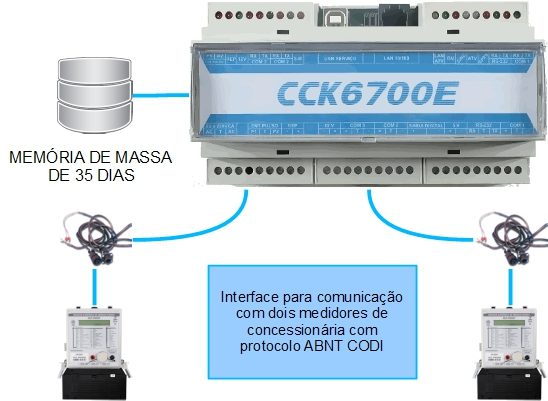
\includegraphics[width=0.8\linewidth]{imagens/cck6700e-esquema.jpg}
    \caption*{Fonte: \citeonline{cck6700E}}
    \label{fig:my_label}
\end{figure}

Feita essa comunicação com medidor, a comunicação do CCK 6700E com o mestre pode ser feito por:
\begin{itemize}
    \item Cabo UTP - É feita a conexão direta entre o dispositivo e o \textit{Switch} com a porta configurada para a VLAN da rede \textit{Modbus}
    \item Fibra Ótica - Através de um conversor de mídia o medidor é conectado à rede por fibra ótica onde na outra extremidade é usado outro conversor para receber a fibra e converter para UTP novamente
    \item Comunicação por Rádio - Um dispositivo recebe os sinais dos medidores através do protocolo RS485, enviando os dados por rádio frequência até outro dispositivo que recebe esse sinal e envia para um dispositivo CCK 7010W que faz a conversão de comunicação serial para Ethernet.
\end{itemize}

\section{Medição Interna}

Cada medidor de fronteira das unidades consumidoras fornece energia para um ou mais prédios de determinada região, sendo assim para um monitoramento mais preciso, faz-se necessário a implantação de subsistemas de medição específicos para cada edificação ou até mesmo em cenários onde se quer ter um controle sobre um consumo mais específico, pode-se ser instalado um medidor em um circuito mais fechado.

O dispositivo responsável por essa medição é o CCK 4400ME, fazendo a leitura e enviando através dos três modos citados na seção \ref{sec:medicao-de-fronteira}. Esse aparelho também possui memória de massa para armazenamento de até 35 dias de leitura.

Além da medição de prédios e equipamentos específicos, o CCK 4400ME é responsável por fazer a leitura de geração dos sistemas de placas fotovoltaicas dos blocos da Universidade. Essa medição é feita através de conexão com a saída do inversor do sistema gerador, enviando os dados para o mestre da rede através dos 3 tipos de comunicação disponíveis.

\section{Diagrama Esquemático Infraestrutura da Rede}

Descrito os modos de medição e comunicação dos diferentes pontos da rede, pode-se resumir todos os modos de conexão utilizados para os vários cenários da rede de medições através do diagrama esquemático abaixo:
\newline

\begin{figure}[H]
    \centering
    \caption{Diagrama Esquemático Rede Modbus de Monitoramento da Universidade Federal de Goiás}
    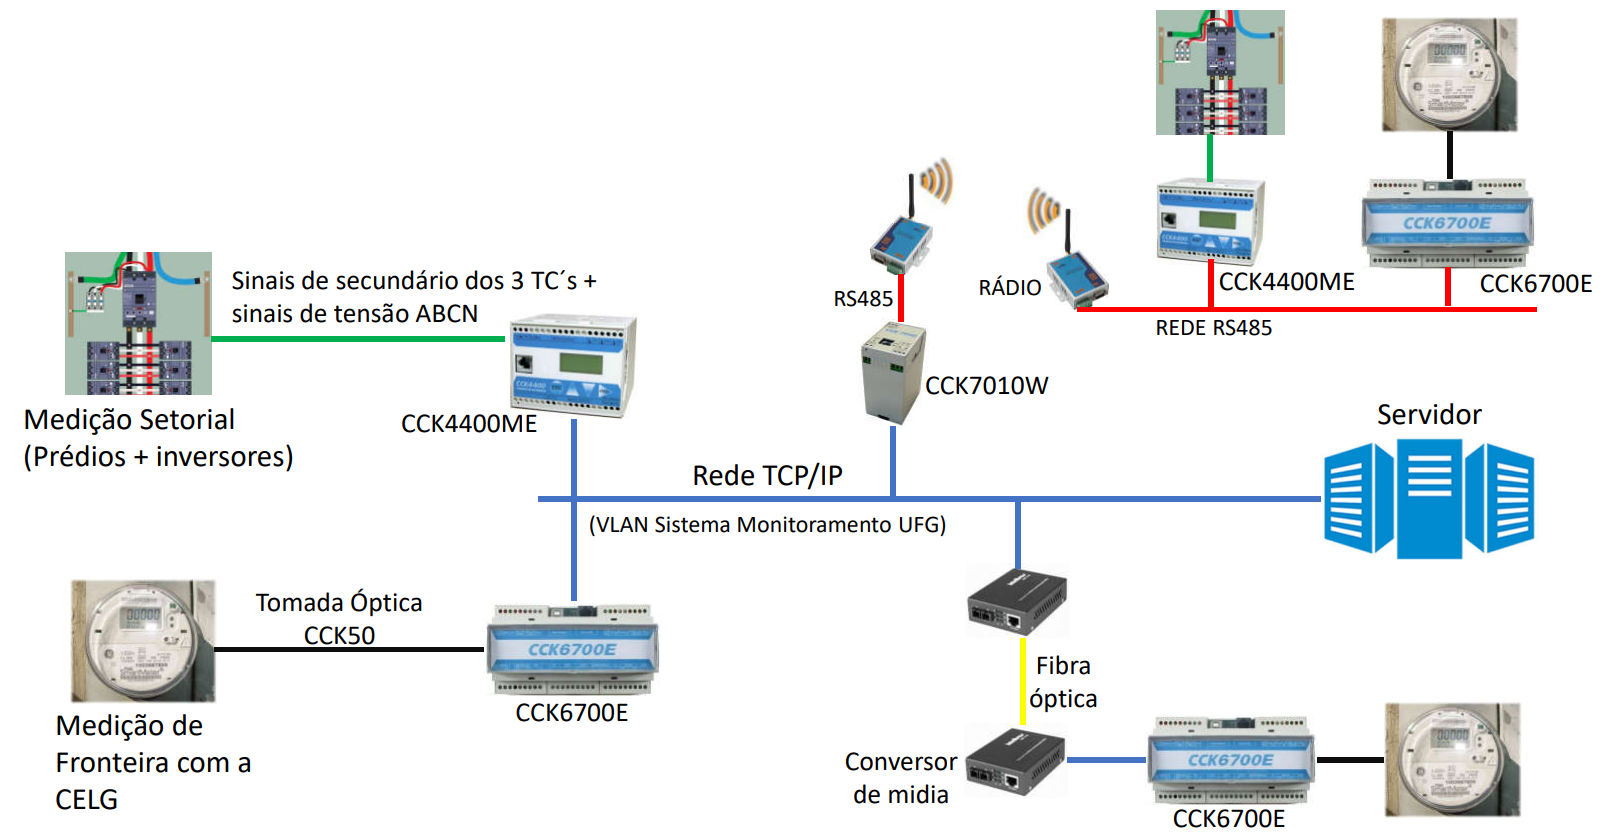
\includegraphics[width=\linewidth]{imagens/esquema-rede-modbus.png}
    \label{fig:diagrama-rede-ufg}
\end{figure}

\chapter{Estrutura de Banco de Dados}
\label{c:estrutura_de_banco_de_dados}
% ---
Descrito o Sistema de infraestrutura da rede, é necessário que os dados dos medidores sejam armazenados para possibilitar consultas futuras. Para isso foi desenvolvida uma estrutura de dados onde pode-se armazenar os dados dos medidores e de suas respectivas medições.Além disso, outro requisito do sistema era que os dados referente às unidades consumidoras pudessem ser armazenados, bem como os dados das suas faturas geradas pela concessionária de energia, com os valores oficiais de medição e cobrança.

Abaixo pode-se observar o layout do modelo de dados com as entidades principais do projeto e seus atributos, bem como suas relações.

\begin{figure}[H]
    \centering
    \caption{Diagrama do Modelo de Dados SIDE}
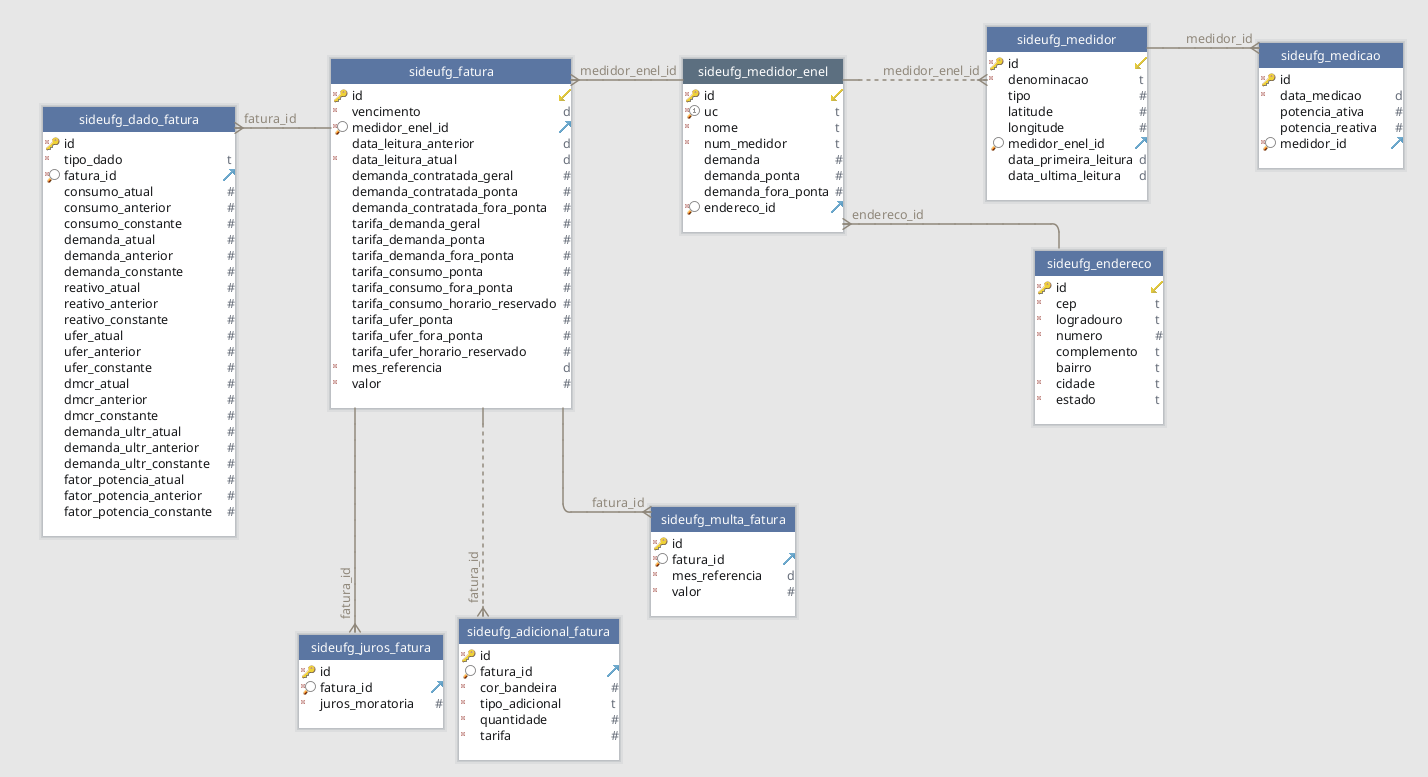
\includegraphics[width=\linewidth]{imagens/modelo-de-dados-side.png}
    \caption*{Fonte: Próprio Autor}
    \label{fig:diagrama-modelo-dados}
\end{figure}

A modelagem da figura \ref{fig:diagrama-modelo-dados}, pode ser visualizada através de um modelo online criado no \textit{software DbSchema}, acessível através do link disponível no apêndice \ref{a:PFC1}.


Devido ao uso de um \textit{framework} para desenvolvimento ágil não se fez necessário preocupar-se com as estruturas de dados referentes a acessos dos usuários, cadastro, definição de papéis, preferências de acesso, bem como criação de versionamento para a criação de um histórico de alteração dos dados do banco. Na figura acima foram omitidas todas as tabelas criadas pelo \textit{framework} Cuba, com a finalidade de focar o modelo no problema específico da aplicação. Toda a documentação referente ao \textit{framework} pode ser encontrada em seu \textit{site} oficial.

\section{Tabela de Medidores da Concessionária}

A tabela onde é feito o cadastro dos Medidores da Concessionária é a tabela \textbf{sideufg\_medidor\_enel} onde os registros são identificados através do campo \textbf{id} do tipo UUID.

Nesta tabela são armazenados os seguintes campos:

\begin{itemize}
    \item \textbf{uc} - Campo obrigatório do tipo \textit{varchar(20)} para armazenar a número da Unidade Consumidora;
    \item \textbf{nome} - Campo obrigatório do tipo \textit{varchar(100)} para armazenar uma denominação para o Medidor;
    \item \textbf{num\_medidor} - Campo obrigatório do tipo \textit{varchar(20)} para armazenar o número do medidor daquele ponto de medição;
    \item \textbf{demanda} - Campo do tipo \textit{integer} para armazenar a demanda contratada para aquela Unidade Consumidora quando a mesma não possui contrato específico por período de medição;
    \item \textbf{demanda\_ponta} - Campo do tipo \textit{integer} para armazenar a demanda contratada para aquela Unidade Consumidora no período de ponta;
    \item \textbf{demanda\_fora\_ponta} - Campo do tipo \textit{integer} para armazenar a demanda contratada para aquela Unidade Consumidora no período fora de ponta;
    \item \textbf{endereco\_id} - Campo do tipo UUID com uma chave estrangeira para armazenar a chave primária do endereço relacionado àquele medidor;
\end{itemize}

\section{Tabela de Medidores da UFG}

A tabela onde é feito o cadastro dos Medidores da CCK é a tabela \textbf{sideufg\_medidor} onde os registros são identificados através do campo \textbf{id} do tipo UUID.
\newpage
Nesta tabela são armazenados os seguintes campos:

\begin{itemize}
    \item \textbf{denominacao} - Campo obrigatório do tipo varchar(255) para armazenar uma denominação para o Medidor;
    \item \textbf{tipo} - Campo do tipo \textit{integer} para armazenar o tipo do medidor podendo ser:
    \subitem 10 - CCK 4400ME;
    \subitem 20 - CCK 6700E;
    \item \textbf{latitude} - Campo do tipo \textit{float8} para armazenar a latitude do medidor para georreferenciamento;
    \item \textbf{longitude} - Campo do tipo \textit{float8} para armazenar a longitude do medidor para georreferenciamento;
    \item \textbf{medidor\_enel\_id} - Campo do tipo UUID com uma chave estrangeira para armazenar a chave primária da unidade consumidora relacionada àquele medidor;
    \item \textbf{data\_primeira\_leitura} - Campo do tipo \textit{timestamp} para armazenar o momento a partir do qual o medidor começou a enviar dados para a base;
    \item \textbf{data\_ultima\_leitura} - Campo do tipo \textit{timestamp} para armazenar o momento da última leitura que o \textit{SIDE Synchronizer} obteve do medidor;
    
\end{itemize}

\section{Tabela de Medições}

A tabela onde é feito o cadastro das medições feitas pelos dispositivos da CCK é a tabela \textbf{sideufg\_medicao} onde os registros são identificados através do campo \textbf{id} do tipo UUID.

Nesta tabela são armazenados os seguintes campos:

\begin{itemize}
    \item \textbf{data\_medicao} - Campo do tipo \textit{timestamp} para armazenar o momento no qual o medidor fez o registro da medição em sua memória de massa;
    \item \textbf{potencia\_ativa} - Campo do tipo \textit{float8} para armazenar o valor de potencia ativa medido;
    \item \textbf{potencia\_reativa} - Campo do tipo \textit{float8} para armazenar o valor de potencia reativa medido;
    \item \textbf{medidor\_id} - Campo do tipo UUID com uma chave estrangeira para armazenar a chave primária do medidor CCK relacionado àquela medição;
\end{itemize}

\section{Tabela de Endereços}

A tabela onde é feito o cadastro dos Endereços das Unidades Consumidoras da UFG é a tabela \textbf{sideufg\_endereco} onde os registros são identificados através do campo \textbf{id} do tipo UUID.

Nesta tabela são armazenados os seguintes campos:

\begin{itemize}
    \item \textbf{cep} - Campo obrigatório do tipo \textit{varchar(8)} para armazenar o CEP do endereço;
    \item \textbf{logradouro} - Campo obrigatório do tipo \textit{varchar(100)} para armazenar o logradouro do endereço;
    \item \textbf{numero} - Campo obrigatório do tipo \textit{integer} para armazenar o número do endereço;
    \item \textbf{complemento} - Campo do tipo \textit{varchar(100)} para armazenar o complemento do endereço;
    \item \textbf{bairro} - Campo do tipo \textit{varchar(100)} para armazenar o bairro do endereço;
    \item \textbf{cidade} - Campo obrigatório do tipo \textit{varchar(100)} para armazenar a cidade do endereço;
    \item \textbf{estado} - Campo obrigatório do tipo \textit{varchar(50)} para armazenar a sigla do estado do endereço, onde a busca pela sigla ocorre através de uma seleção no cadastro através de um \textit{enumeration};
    
\end{itemize}

\section{Estrutura de Dados para Armazenamento das Faturas}

As faturas energéticas das unidades consumidoras possuem um grande volume de dados que são importantes para as análises econômicas, quantitativas e qualitativas do consumo das edificações da Universidade. Desde os dados financeiros como valor, tarifas individuais, adicionais tarifários, contratos de demanda, até dados referentes ao consumo propriamente dito com as leituras nos horários específicos de ponta, fora de ponta e horário reservado.

Para a modelagem dessa estrutura de dados foi pensado em uma divisão em cinco tabelas, sendo uma tabela principal contendo os principais dados da fatura, e quatro auxiliares contendo desde dados esporádicos como multa e juros até dados repetitivos como as várias leituras de demanda, consumo, UFER, entre outros na fatura.

\newpage

As tabelas criadas referente ao armazenamento das faturas estão listadas abaixo e serão detalhadas nas sub-sessões \ref{sub:tabela-fatura}, \ref{sub:tabela-dado-fatura}, \ref{sub:tabela-adicional-fatura}, \ref{sub:tabela-multa-fatura} e \ref{sub:tabela-juros-fatura}:

\begin{itemize}
    \item sideufg\_fatura;
    \item sideufg\_dado\_fatura;
    \item sideufg\_adicional\_fatura;
    \item sideufg\_multa\_fatura;
    \item sideufg\_juros\_fatura;
\end{itemize}

\subsection{Tabela de Faturas}
\label{sub:tabela-fatura}

A tabela onde é feito o cadastro das faturas de cada Unidade Consumidora é a tabela \textbf{sideufg\_fatura} onde os registros são identificados através do campo \textbf{id} do tipo UUID.

Nesta tabela são armazenados os seguintes campos:

\begin{itemize}
    \item \textbf{vencimento} - Campo obrigatório do tipo \textit{date} para armazenar a data de vencimento da fatura;
    \item \textbf{medidor\_enel\_id} - Campo obrigatório do tipo UUID com uma chave estrangeira para armazenar a chave primária da unidade consumidora relacionada àquela fatura;
    \item \textbf{data\_leitura\_anterior} - Campo do tipo \textit{date} para armazenar a data da leitura da fatura anterior;
    \item \textbf{data\_leitura\_atual} - Campo obrigatório do tipo \textit{date} para armazenar a data da leitura atual da fatura;
    \item \textbf{demanda\_contratada\_geral} - Campo do tipo \textit{integer} para armazenar a demanda contratada naquele mês para aquela Unidade Consumidora quando a mesma não possui contrato específico por período de medição;
    \item \textbf{demanda\_contratada\_ponta} - Campo do tipo \textit{integer} para armazenar a demanda contratada naquele mês para aquela Unidade Consumidora no período de ponta;
    \item \textbf{demanda\_contratada\_fora\_ponta} - Campo do tipo \textit{integer} para armazenar a demanda contratada naquele mês para aquela Unidade Consumidora no período fora de ponta;
    \item \textbf{tarifa\_demanda\_geral} - Campo do tipo \textit{big decimal (19,6)} para armazenar a tarifa da demanda geral naquele mês;
    \item \textbf{tarifa\_demanda\_ponta} - Campo do tipo \textit{big decimal (19,6)} para armazenar a tarifa da demanda no horário de ponta naquele mês;
    \item \textbf{tarifa\_demanda\_fora\_ponta} - Campo do tipo \textit{big decimal (19,6)} para armazenar a tarifa da demanda no horário fora de ponta naquele mês;
    \item \textbf{tarifa\_consumo\_ponta} - Campo do tipo \textit{big decimal (19,6)} para armazenar a tarifa do consumo no horário de ponta naquele mês;
    \item \textbf{tarifa\_consumo\_fora\_ponta} - Campo do tipo \textit{big decimal (19,6)} para armazenar a tarifa do consumo no horário fora de ponta naquele mês;
    \item \textbf{tarifa\_consumo\_horario\_reservado} - Campo do tipo \textit{big decimal (19,6)} para armazenar a tarifa do consumo no horário reservado naquele mês;
    \item \textbf{tarifa\_ufer\_ponta} - Campo do tipo \textit{big decimal (19,6)} para armazenar a tarifa da UFER no horário de ponta naquele mês;
    \item \textbf{tarifa\_ufer\_fora\_ponta} - Campo do tipo \textit{big decimal (19,6)} para armazenar a tarifa da UFER no horário fora de ponta naquele mês;
    \item \textbf{tarifa\_ufer\_horario\_reservado} - Campo do tipo \textit{big decimal (19,6)} para armazenar a tarifa da UFER no horário reservado naquele mês;
    \item \textbf{mes\_referencia} - Campo obrigatório do tipo \textit{date} para armazenar o mês de referência da fatura;
    \item \textbf{valor} - Campo obrigatório do tipo \textit{big decimal (19,2)} para armazenar o valor final da fatura;
\end{itemize}

\subsection{Tabela dos Dados da Fatura}
\label{sub:tabela-dado-fatura}
A tabela onde é feito o cadastro dos dados específicos da fatura adquiridos pela interpretação da tabela da segunda página das faturas como a do exemplo da imagem abaixo é a tabela  \textbf{sideufg\_dado\_fatura} onde os registros são identificados através do campo \textbf{id} do tipo UUID.

\begin{figure}[H]
    \centering
    \caption{Modelo de Tabela de Dados Específicos da Fatura}
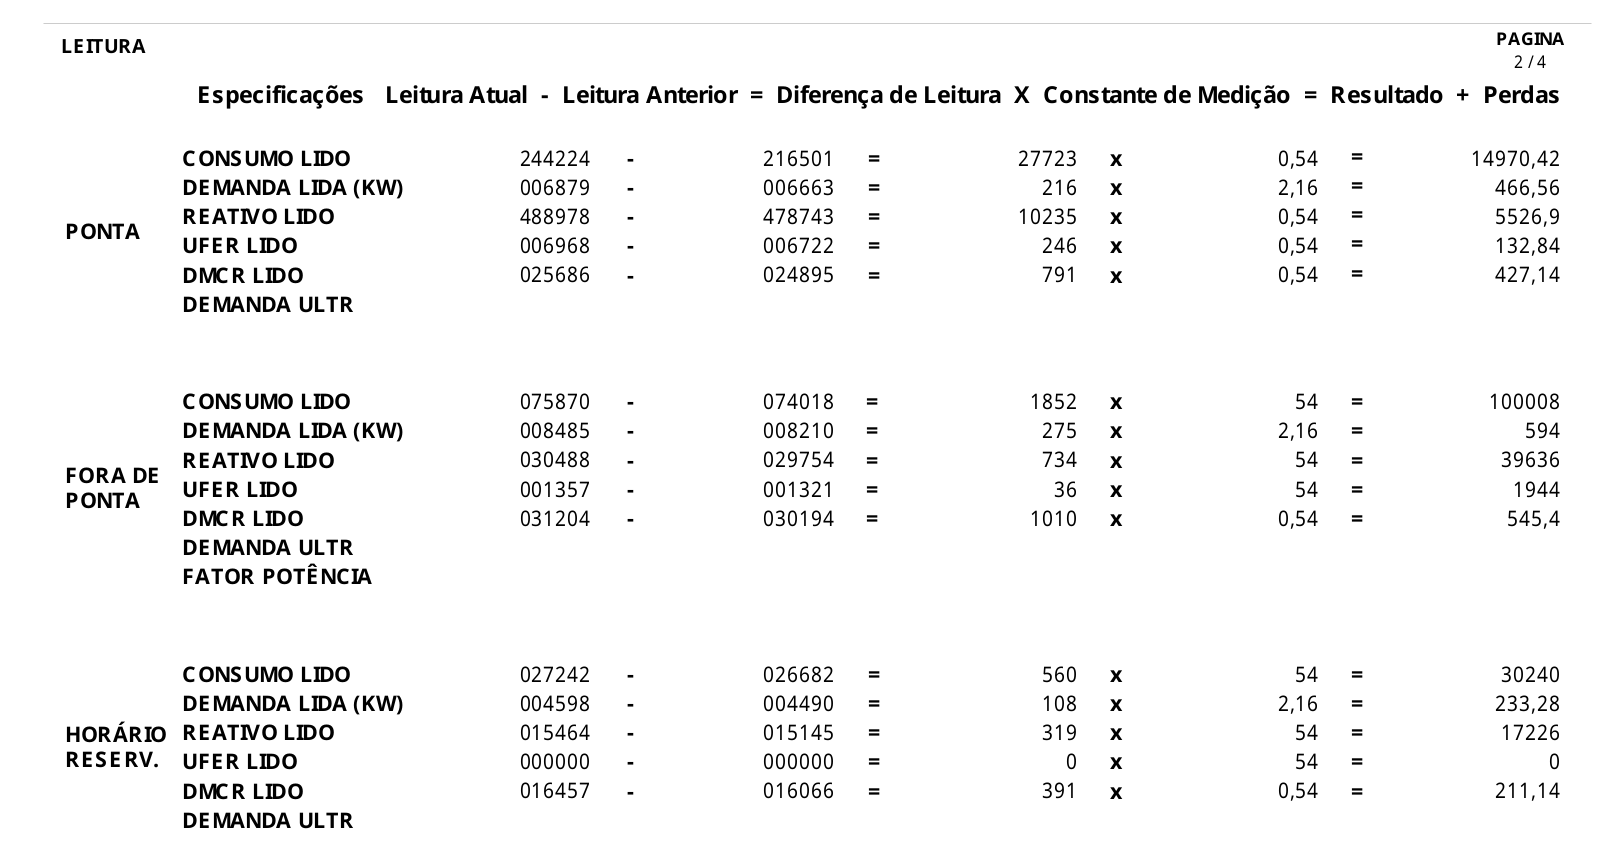
\includegraphics[width=0.8\linewidth]{imagens/modelo-tabela-dados-fatura.png}
    \caption*{Fonte: Próprio Autor}
    \label{fig:modelo-tabela-dados-fatura}
\end{figure}

Nesta tabela são armazenados os seguintes campos:

\begin{itemize}
    \item \textbf{tipo\_dado} - Campo obrigatório do tipo \textit{varchar(50)} para armazenar o tipo da leitura, podendo ser:
    \subitem P - Ponta;
    \subitem F - Fora de Ponta;
    \subitem H - Horário Reservado;
    \item \textbf{fatura\_id} - Campo obrigatório do tipo UUID com uma chave estrangeira para armazenar a chave primária da fatura relacionada àquele dado;
    
    \item \textbf{consumo\_atual} - Campo do tipo \textit{integer} para armazenar a leitura atual de consumo do dado da fatura;
    \item \textbf{consumo\_anterior} - Campo do tipo \textit{integer} para armazenar a leitura anterior de consumo do dado da fatura;
    \item \textbf{consumo\_constante} - Campo do tipo \textit{float8} para armazenar a constante de medição do consumo do dado da fatura;
    
    \item \textbf{demanda\_atual} - Campo do tipo \textit{integer} para armazenar a leitura atual de demanda do dado da fatura;
    \item \textbf{demanda\_anterior} - Campo do tipo \textit{integer} para armazenar a leitura anterior de demanda do dado da fatura;
    \item \textbf{demanda\_constante} - Campo do tipo \textit{float8} para armazenar a constante de medição da demanda do dado da fatura;
    
    \item \textbf{reativo\_atual} - Campo do tipo \textit{integer} para armazenar a leitura atual de reativo do dado da fatura;
    \item \textbf{reativo\_anterior} - Campo do tipo \textit{integer} para armazenar a leitura anterior de reativo do dado da fatura;
    \item \textbf{reativo\_constante} - Campo do tipo \textit{float8} para armazenar a constante de medição do reativo do dado da fatura;
    
    \item \textbf{ufer\_atual} - Campo do tipo \textit{integer} para armazenar a leitura atual de consumo de energia reativa do dado da fatura;
    \item \textbf{ufer\_anterior} - Campo do tipo \textit{integer} para armazenar a leitura anterior de consumo de energia reativa do dado da fatura;
    \item \textbf{ufer\_constante} - Campo do tipo \textit{float8} para armazenar a constante de medição do consumo de energia reativa do dado da fatura;
    
    \item \textbf{dmcr\_atual} - Campo do tipo \textit{integer} para armazenar a leitura atual de demanda máxima corrigida do dado da fatura;
    \item \textbf{dmcr\_anterior} - Campo do tipo \textit{integer} para armazenar a leitura anterior de demanda máxima corrigida do dado da fatura;
    \item \textbf{dmcr\_constante} - Campo do tipo \textit{float8} para armazenar a constante de medição da demanda máxima corrigida  do dado da fatura;
    
    \item \textbf{demanda\_ultr\_atual} - Campo do tipo \textit{integer} para armazenar a leitura atual de demanda ultrapassada do dado da fatura;
    \item \textbf{demanda\_ultr\_anterior} - Campo do tipo \textit{integer} para armazenar a leitura anterior de demanda ultrapassada do dado da fatura;
    \item \textbf{demanda\_ultr\_constante} - Campo do tipo \textit{float8} para armazenar a constante de medição da demanda ultrapassada do dado da fatura;
    
    \item \textbf{fator\_potencia\_atual} - Campo do tipo \textit{integer} para armazenar a leitura atual de fator de potência do dado da fatura;
    \item \textbf{fator\_potencia\_anterior} - Campo do tipo \textit{integer} para armazenar a leitura anterior de fator de potência do dado da fatura;
    \item \textbf{fator\_potencia\_constante} - Campo do tipo \textit{float8} para armazenar a constante de fator de potência do dado da fatura;
    
    
\end{itemize}

\subsection{Tabela dos Adicionais Tarifários da Fatura}
\label{sub:tabela-adicional-fatura}

A tabela onde é feito o cadastro dos adicionais tarifários de bandeira de cada fatura é a tabela \textbf{sideufg\_adicional\_fatura} onde os registros são identificados através do campo \textbf{id} do tipo UUID.

Nesta tabela são armazenados os seguintes campos:

\begin{itemize}
    \item \textbf{fatura\_id} - Campo obrigatório do tipo UUID com uma chave estrangeira para armazenar a chave primária da fatura relacionada àquele adicional;
    \item \textbf{cor\_bandeira} - Campo obrigatório do tipo \textit{integer} para armazenar a cor da bandeira do adicional daquele mês para aquela fatura, podendo ser:
    \subitem 1 - Verde;
    \subitem 2 - Amarela;
    \subitem 3 - Vermelha;
    \item \textbf{tipo\_adicional} - Campo obrigatório do tipo \textit{varchar(50)} para armazenar o tipo do adicional tarifário, podendo ser:
    \subitem P - Ponta;
    \subitem F - Fora de Ponta;
    \subitem H - Horário Reservado;
    \item \textbf{quantidade} - Campo obrigatório do tipo \textit{big decimal (13,2)} para armazenar a quantidade do adicional a ser cobrado naquele mês naquela fatura;
    \item \textbf{tarifa} - Campo obrigatório do tipo \textit{big decimal (19,6)} para armazenar a tarifa do adicional a ser cobrado naquele mês naquela fatura;
\end{itemize}

\subsection{Tabela das Multas da Fatura}
\label{sub:tabela-multa-fatura}

A tabela onde é feito o cadastro das multas aplicadas à cada fatura é a tabela \textbf{sideufg\_multa\_fatura} onde os registros são identificados através do campo \textbf{id} do tipo UUID.

Nesta tabela são armazenados os seguintes campos:

\begin{itemize}
    \item \textbf{fatura\_id} - Campo obrigatório do tipo UUID com uma chave estrangeira para armazenar a chave primária da fatura relacionada àquela multa;
    \item \textbf{mes\_referencia} - Campo obrigatório do tipo \textit{date} para armazenar o mês de referência da multa da fatura;
    \item \textbf{valor} - Campo obrigatório do tipo \textit{big decimal (13,2)} para armazenar o valor da multa da fatura;
\end{itemize}

\subsection{Tabela dos Juros da Fatura}
\label{sub:tabela-juros-fatura}

A tabela onde é feito o cadastro dos juros monetários aplicados à cada fatura é a tabela \textbf{sideufg\_juros\_fatura} onde os registros são identificados através do campo \textbf{id} do tipo UUID.

Nesta tabela são armazenados os seguintes campos:

\begin{itemize}
    \item \textbf{fatura\_id} - Campo obrigatório do tipo UUID com uma chave estrangeira para armazenar a chave primária da fatura relacionada àquele juros;
    \item \textbf{juros\_moratoria} - Campo obrigatório do tipo \textit{big decimal (13,2)} para armazenar o valor dos juros da fatura;
\end{itemize}
\chapter{Sistema Sincronizador de Dados}
\label{c:sistema_sincronizador_de_dados}
% ---
Descrita a estrutura de banco de dados do projeto, bem como a infraestrutura da rede \textit{Modbus} de medição da UFG, pode-se entender agora o modo de funcionamento do Sistema Responsável por alimentar o banco com as informações capturadas dos medidores. Para isso foi desenvolvido uma aplicação na linguagem \textit{node js}, que é acionada pelo \textit{crontabs} de um servidor Linux com o acionamento a cada minuto.

O código do \textit{SIDE Synchronizer} é composto basicamente de dois momentos, como mostrado no algoritmo \ref{listing:sidesynchronizer}:

\begin{enumerate}
    \item O sistema acessa o Mestre da rede Modbus e requisita a lista de escravos cadastrados, atualizando o banco de dados com as alterações do mesmo.
    \item O sistema utiliza essa lista de medidores para requisitar as últimas medições feitas em cada medidor a partir da data da última leitura de cada um.
\end{enumerate}

Essas duas etapas serão melhor descritas nas sessões \ref{sec:sincronizacao-medidores} e \ref{sec:sincronizacao-medicoes}, porém, por hora, pode-se analisar o código abaixo da classe principal do \textit{SIDE Synchronizer}.

\begin{listing}[ht]
\caption{Código Principal \textit{SIDE Synchronizer}}
\inputminted[frame=lines, 
    framesep=5mm, fontsize=\footnotesize, linenos=true, label={sidesynchronizer.js}]{js}{codigos/sidesynchronizer.js}
\label{listing:sidesynchronizer}
\end{listing}

Inicialmente, na linha 4 inicializa-se uma lista de medidores que receberá a listagem do método medidores.sincronizaMedidoresCCK() na linha 6. Após o retorno do método e a população do \textit{array}, faz-se a iteração por ele onde a cada iteração é executado o método medicoes.sincronizaMedicoesCCK(medidor) passando o medidor como parâmetro.

\newpage
Após a iteração, na linha 10 se encerra o processo, que em média leva 1,2 segundos para executar na atual situação da planta de medidores da UFG. após 1 minuto o cron do \textit{Linux} chama esse processo novamente, mantendo sempre assim a base atualizada com as medições da rede \textit{Modbus}.

A seguir serão detalhados os dois métodos que fazem a sincronização dos medidores e suas respectivas medições.

\section{Sincronização de Medidores}
\label{sec:sincronizacao-medidores}

Descrito o funcionamento Geral da aplicação, pode-se analisar o código resumido abaixo, da classe responsável pela sincronização inicial dos medidores, como descrito no algoritmo \ref{listing:medidores}.

\begin{listing}[ht]
\caption{Código Resumido da Classe de Medidores}
\inputminted[
    frame=lines, 
    framesep=5mm, 
    fontsize=\footnotesize, 
    linenos=true, 
    label={medidores.js}, 
    firstline=26, 
    lastline=58
    ]{js}{codigos/medidores.js}
\label{listing:medidores}
\end{listing}

O método sincronizaMedidoresCCK faz inicialmente uma listagem de todos os medidores cadastrados na rede e os armazena na variável medidoresCCK, onde na linha 38 inicializa-se uma lista de retornos da consulta que será populada com os medidores cadastrados na rede \textit{Modbus}. Na linha 40 é feita uma requisição http padrão na  Após o retorno do método e a população do \textit{array}, faz-se a iteração por ele onde a cada iteração é executado o método medicoes.sincronizaMedicoesCCK(medidor) passando o medidor como parâmetro. 

Após a listagem, é feita no servidor CCK uma outra validação, onde ma linha 29 após passar os medidores se obtém para cada um a data da última e da primeira leitura que o dispositivo fez, atualizando assim mais uma vez a lista medidoresCCK. 

Após o preenchimento é buscado no banco de dados os medidores já registrados e feito o cadastro caso não existam na base, e atualização da denominação, e datas de primeira e ultima leitura caso já existam na base. Ao final é retornado a lista de medidores atualizada.

\section{Sincronização de Medições}
\label{sec:sincronizacao-medicoes}

Após o retorno da sincronização dos medidores fornecer a lista atualizada de medidores, pode-se iterar essa lista chamando-se, para cada medidor, a sincronização de medições exibida no algoritmo \ref{listing:medicoes}.

\begin{listing}[ht]
\caption{Código Resumido da Classe de Medições}
\inputminted[
    frame=lines, 
    framesep=5mm, 
    fontsize=\footnotesize, 
    linenos=true, 
    label={medicoes.js}, 
    firstline=19, 
    lastline=32
    ]{js}{codigos/medicoes.js}
\label{listing:medicoes}
\end{listing}

\newpage

Inicialmente, na linha 21 é feita uma busca no banco pela última medição do medidor, e posteriormente é feita a seguinte validação: se a data de medição da última leitura não for nula é feita uma busca das últimas leituras existentes no servidor a partir daquela data, caso contrário, entende-se que não existem leituras na tabela de medições para aquele medidor e é feita uma busca por todas as leituras daquele escravo no servidor. 

Após a busca das medições caso ela apresente retorno, as medições são inseridas no banco para este medidor. Este processo é iterado para todos os medidores existentes e após isso a execução do sincronizador é finalizada.
\chapter{Sistema Interpretador de Faturas} 
\label{c:sistema_interpretador_de_faturas}
% ---
Descrita a parte de obtenção dos dados dos medidores, uma outra importante fonte de dados, principalmente econômicos, são as faturas de energia, porém devido ao grande número de unidades consumidoras da UFG essa análise e obtenção dos dados apenas de maneira manual seria algo com um alto custo, por isso, foi desenvolvido um sistema capaz de fazer uma carga em massa das faturas, que fosse capaz de interpretar os dados e gerar um resultado para análise tanto por softwares de \textit{business intelligence} tanto como poder alimentar o banco de dados do SIDE.

Este sistema pode ser executado independente do sistema operacional por se tratar de uma aplicação java, que é multiplataforma, e de maneira independente do banco de dados, sendo capaz de gerar um arquivo CSV com os dados extraídos das faturas contidas em um diretório selecionado e seus sub-diretórios, além de ser possível a alimentação do banco quando o dispositivo no qual for executado, tiver acesso a rede e os dados de acesso ao banco de dados do SIDE. A figura \ref{fig:pdf-reader} segue uma captura da tela do sistema \textit{PdfReader}:

\begin{figure}[H]
    \centering
    \caption{Tela Principal do Sistema PdfReader}
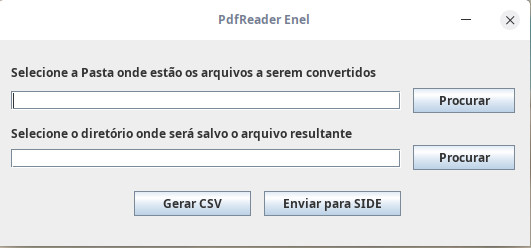
\includegraphics[width=\linewidth]{imagens/pdf-reader.png}
\caption*{Fonte: Próprio Autor}
\label{fig:pdf-reader}
\end{figure}

\newpage
\section{Processo de Interpretação da Fatura}

Após selecionado o diretório de origem e o de destino do arquivo resultante, ao clicar em um dos dois botões de ação é executado o código do algoritmo \ref{listing:pdfReader}:

\begin{listing}[ht]
\caption{Código Principal \textit{PdfReader}}
\inputminted[frame=lines,
    firstline=26,
    lastline=52,
    framesep=5mm, fontsize=\footnotesize, linenos=true, label={App.java}]{java}{codigos/PdfReader/App.java}
\label{listing:pdfReader}
\end{listing}

Inicialmente é criado um arquivo temporário para armazenamento das conversões de PDF para texto puro das faturas, após é inicializado uma \textit{Collection} com todos os arquivos dentro do diretório passado como parâmetro através da variável \textit{path}, e esses arquivos são iterados fazendo inicialmente em cada arquivo a validação se o mesmo é um arquivo com a extensão PDF após isso é feita interpretação da primeira página da fatura onde, dependendo da opção selecionada será carregado o CSV ou o banco com esses dados coletados.

Após a leitura da primeira página o mesmo processo ocorre para a segunda página, e assim sucessivamente até todos os arquivos terem sido lidos, retornando para a tela principal com a mensagem de leitura efetivada com sucesso.r
\chapter{Interface de Usuário}
\label{c:interface_de_usuario}
% ---
Todo o sistema para alimentação dos dados de consumo, bem como a estrutura dos dados em si está definida, porém falta um sistema capaz se possibilitar uma visualização real pelo usuário dos dados coletas, bem como uma interface que permita que sejam cadastrados dados de gerenciamento dos dispositivos de medição.

Para isso foi desenvolvida a interface \textit{web} do SIDE, como sendo a interface principal do sistema, sendo ela a responsável por cadastro de usuários para a utilização do sistema, visualização dos dados de medição dos medidores CCK, cadastro das unidades consumidoras, visualização georreferenciada dos dispositivos instalados, entre outras.

\section{Uso do \textit{CUBA Framework}}

Para o desenvolvimento da Interface do SIDE, foi escolhida a linguagem de programação Java com o uso de um \textit{framework} que possibilitasse o desenvolvimento ágil facilitando na criação das entidades e seus respectivos relacionamentos e desse base para a criação de uma boa visualização para o usuário. 

A plataforma escolhida para desenvolvimento foi o \textit{CUBA Framework}, utilizado em sua versão 6.10 cuja a documentação pode ser acessada através do anexo \ref{anex:doc-cuba}.

A interface de usuário disponibilizada pelo CUBA pode ser tanto uma interface padrão utilizando \textit{Spring} quando uma interface mais personalizável utilizando \textit{Polymer 2}, que é um framework JavaScript da empresa Google para desenvolvimento web baseado na utilização de \textit{Web Components}, que foi a escolhida para o desenvolvimento deste projeto.

\section{Uso da biblioteca \textit{Polymer 2}}

Escolhida a Interface de uso Polymer precisa-se entender melhor os padrões de desenvolvimento que a mesma utiliza.

O Polymer é uma biblioteca JavaScript usada para a criação de aplicações web usando o conceito de \textit{Web Components}. Esses \textit{Web Components} podem ser descritos como elementos reutilizáveis que podem ser inseridos em páginas ou aplicações \textit{web}, podendo inclusive ser mesclado com outras bibliotecas JavaScript. O Polymer é como um bloco de montar, que pode ser encaixado de diversas maneiras para construir diferentes tipos de aplicações. 

Nesta versão do CUBA é utilizada a versão 2 do Polymer, cuja a documentação pode ser acessada através do anexo \ref{anex:doc-polymer}.

\section{Telas do SIDE}

Descrito os frameworks utilizados, pode-se agora definir os modos de funcionamento das telas desenvolvidas para o sistema. 

\subsection{Login}

A tela inicial do sistema é a tela de login, mostrada na figura \ref{fig:side-login}, sendo responsável pela autenticação do usuário cadastrado no sistema, gerando uma chave de sessão válida para o mesmo, liberando assim o seu acesso ao sistema.

Esta tela permite também a troca da senha atual do usuário, enviando uma nova senha temporária para o endereço de e-mail cadastrado para o mesmo. Abaixo temos uma imagem da tela de login.

\begin{figure}[H]
    \centering
    \caption{Tela de Login do SIDE}
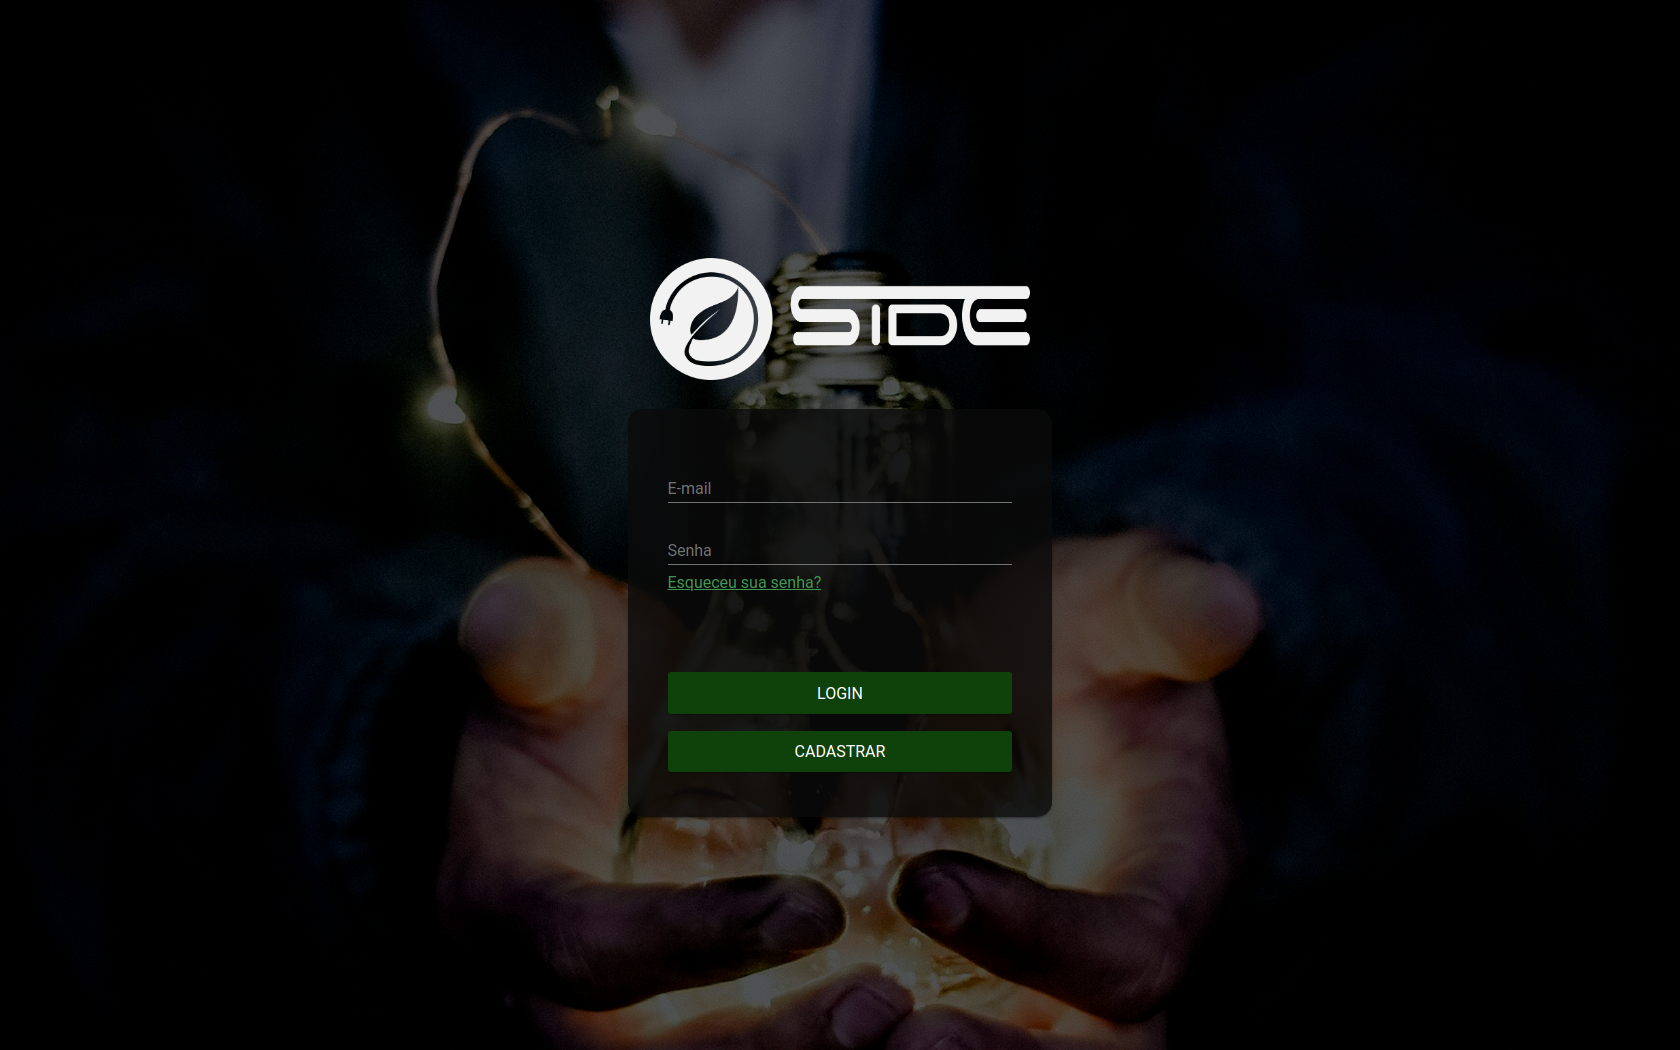
\includegraphics[width=\linewidth]{imagens/side/side-login.png}
    \caption*{Fonte: Próprio Autor}
    \label{fig:side-login}
\end{figure}

Além disso caso não possua acesso ainda, pode ser feito o cadastro do usuário, fornecendo seu nome, e-mail, cpf, e a senha desejada. Este cadastro irá gerar um acesso básico ao sistema que poderá ser controlado pelo administrador do sistema. Na figura \ref{fig:side-cadastro} temos uma imagem da tela de cadastro.

\begin{figure}[H]
    \centering
    \caption{Tela de Cadastro do SIDE}
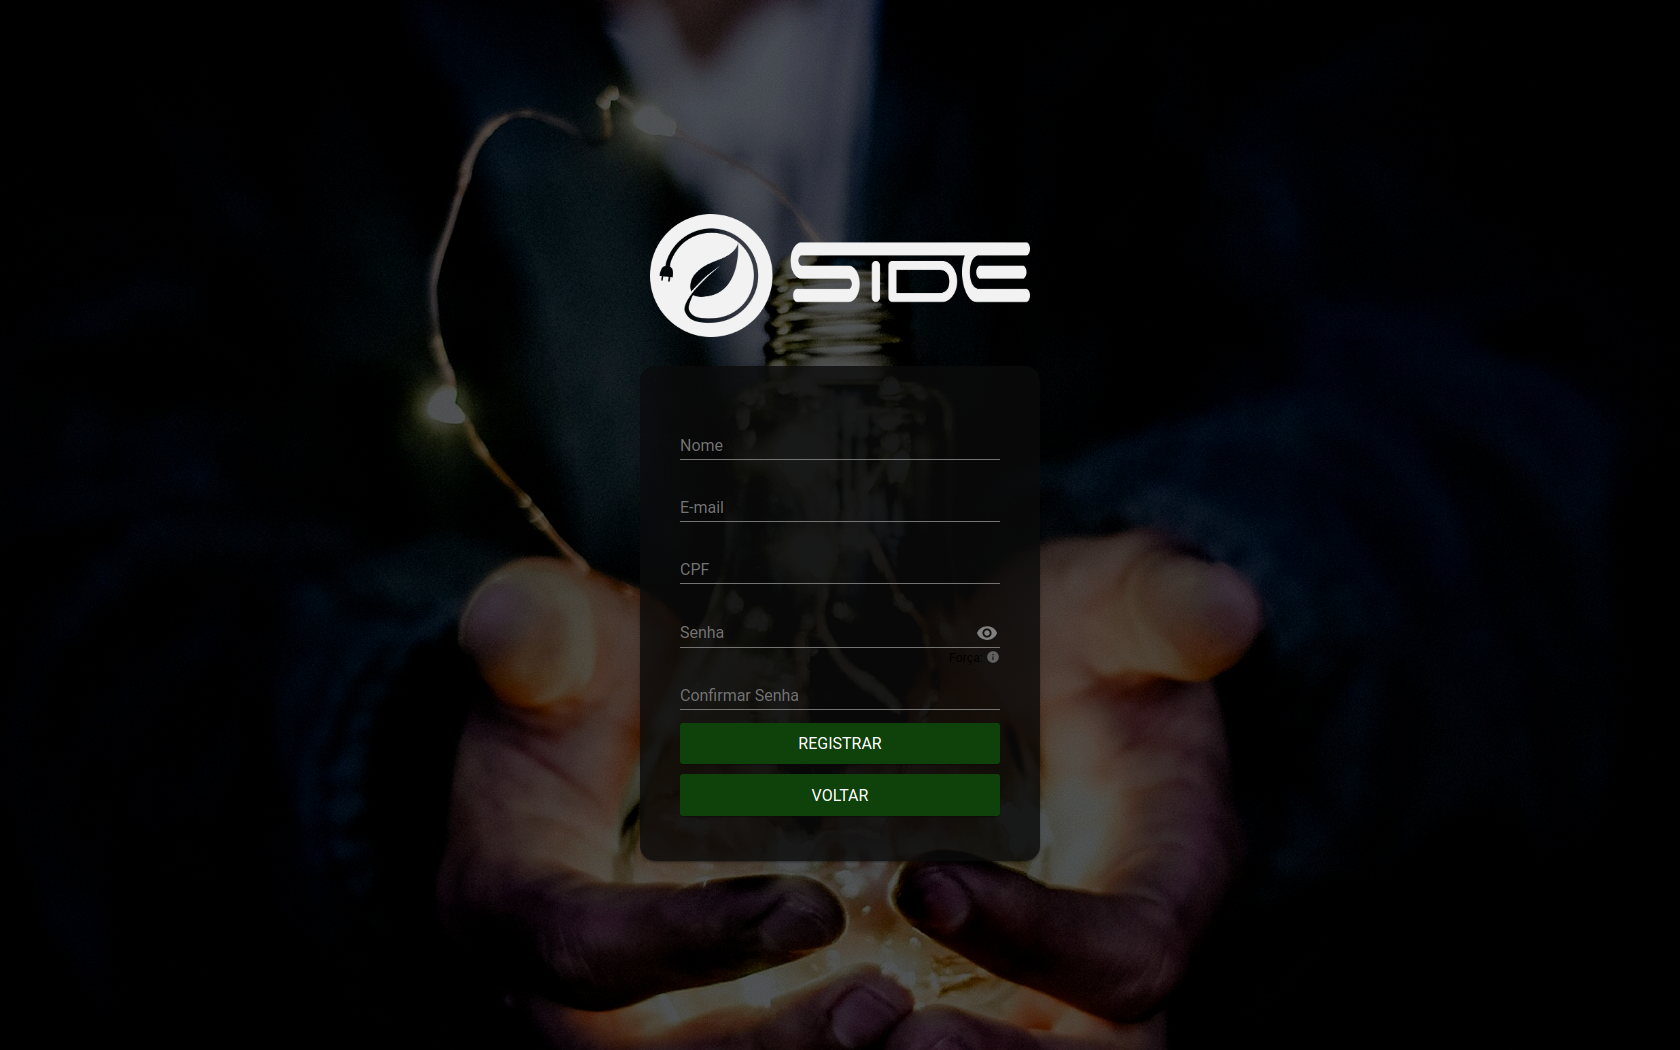
\includegraphics[width=0.65\linewidth]{imagens/side/side-cadastro.png}
    \caption*{Fonte: Próprio Autor}
    \label{fig:side-cadastro}
\end{figure}

\subsection{Tela Principal}

Após autenticado no sistema o usuário tem acesso ao uso do SIDE, onde inicialmente ele verá um mapa com todos os pontos de medição cadastrado no sistema que possuam suas coordenadas geográficas cadastradas. Esses pontos podem ser clicados, fornecendo informações mais detalhadas como consumo atual através da última leitura, denominação, data da última leitura, unidade consumidora vinculada à ele, e o tipo de medidor.

O mapa foi construído em cima de um \textit{Web Component} do Polymer fornecido pela Google para acesso a api do Google Maps. Na figura \ref{fig:side-home} temos uma imagem da \textit{home} do sistema.

\begin{figure}[H]
    \centering
    \caption{Tela Principal do SIDE}
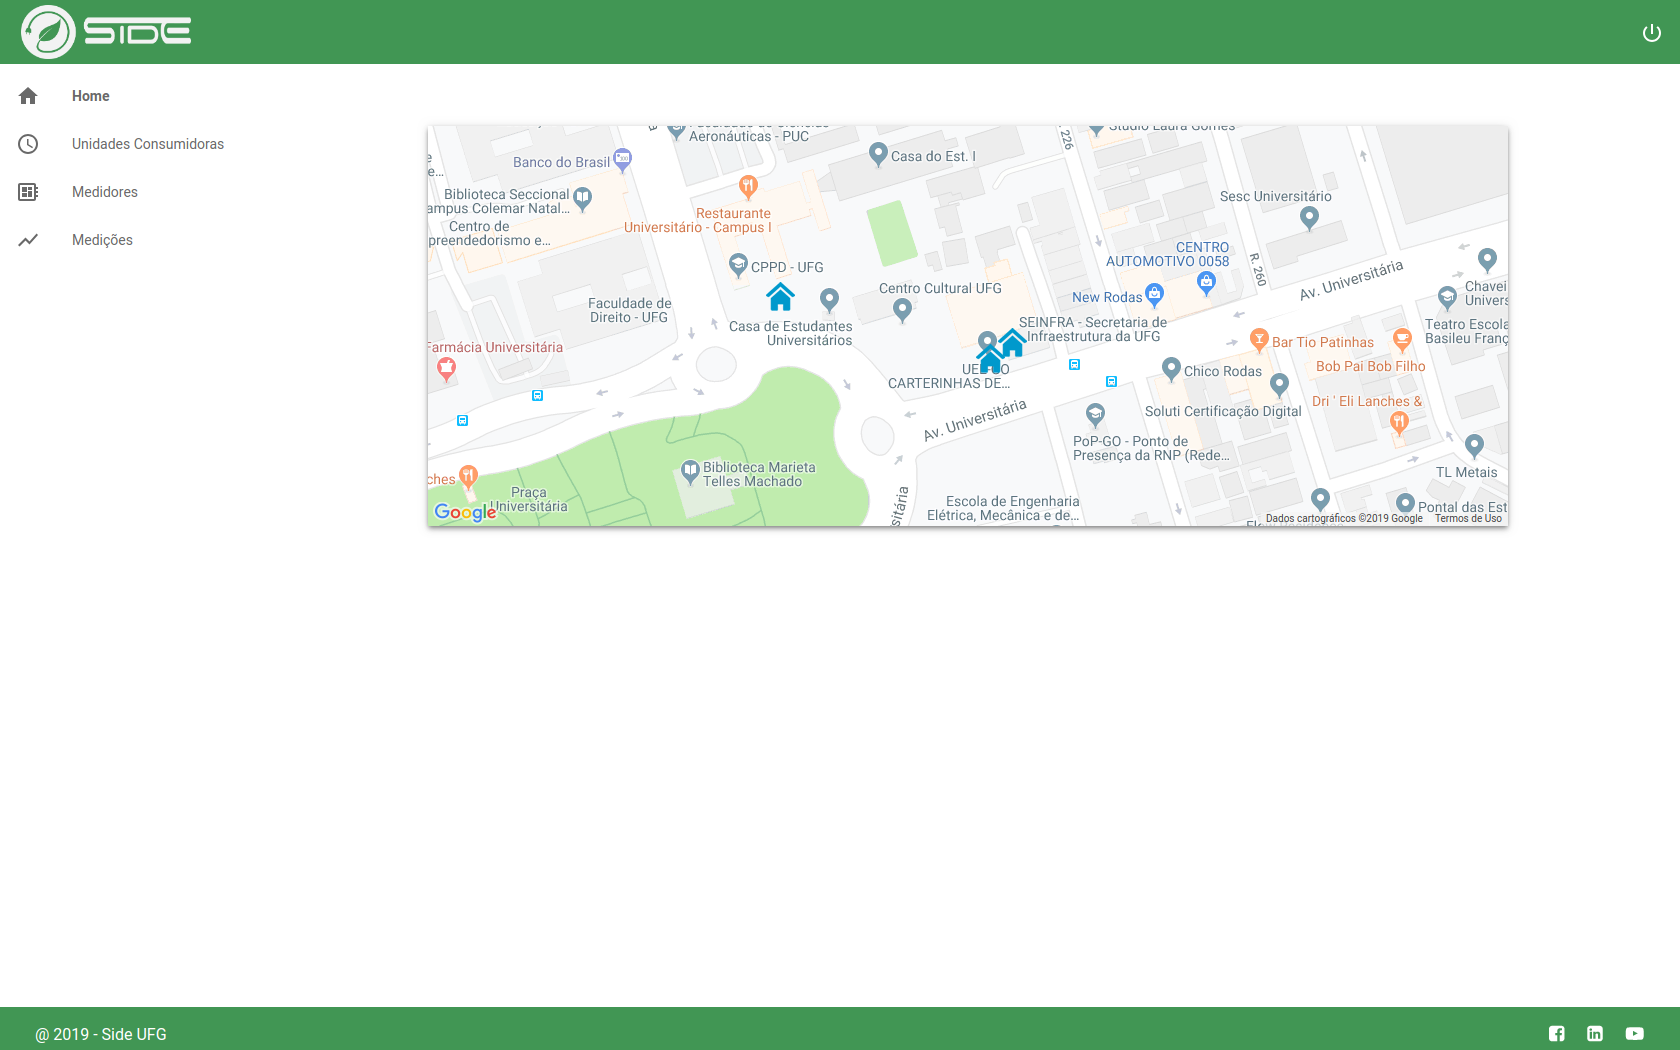
\includegraphics[width=0.65\linewidth]{imagens/side/side-home.png}
    \caption*{Fonte: Próprio Autor}
    \label{fig:side-home}
\end{figure}


\subsection{Cadastro de Unidades Consumidoras}

No menu de Unidades Consumidoras podemos visualizar os medidores da concessionária cadastrados na base, descriminados pela junção de seu nome com a número da unidade consumidora do mesmo.

Na listagem de cada unidade, pode-se ver o número do medidor e suas demandas contratadas na primeira coluna, e o endereço completo na segunda coluna. Na figura \ref{fig:side-uc-list} temos as ações disponíveis para aquele item, sendo a primeira o \textit{upload} de faturas daquela unidade consumidora, onde esta relação será validada no momento do \textit{upload}, e o segundo ícone, mostra a edição do item em si.

\begin{figure}[H]
    \centering
    \caption{Tela de Listagem das Unidades Consumidoras}
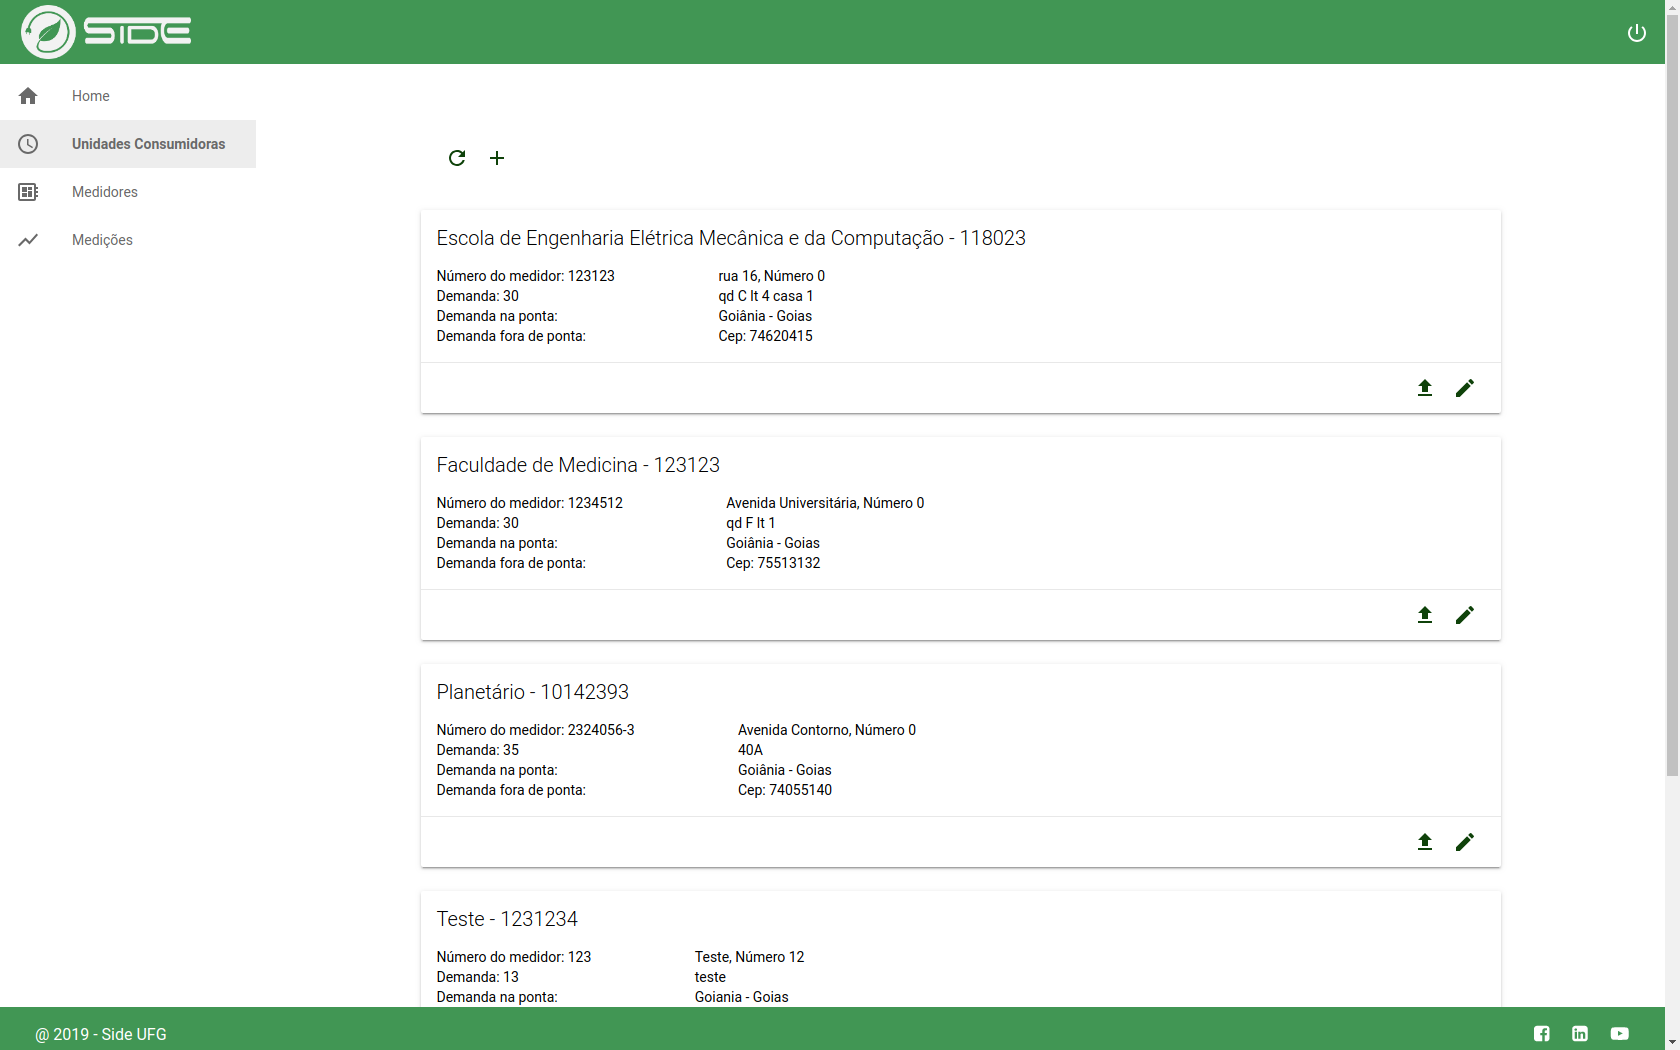
\includegraphics[width=\linewidth]{imagens/side/side-uc-list.png}
    \caption*{Fonte: Próprio Autor}
    \label{fig:side-uc-list}
\end{figure}

Ao criar uma Unidade Consumidora, através do ícone superior da tela ou editar uma através do ícone de edição do item, teremos acesso a tela de edição, onde deverão ser preenchidos os dados e após o preenchimento poderão ser salvos. Além disso é possível na tela de edição de uma unidade consumidora, apagar aquela unidade, onde a nível de banco serão desassociados todos os medidores CCK vinculados àquela unidade. 

\newpage

Na figura \ref{fig:side-uc-edit} temos uma imagem da tela de edição de unidade consumidora:

\begin{figure}[H]
    \centering
    \caption{Tela de Edição das Unidades Consumidoras}
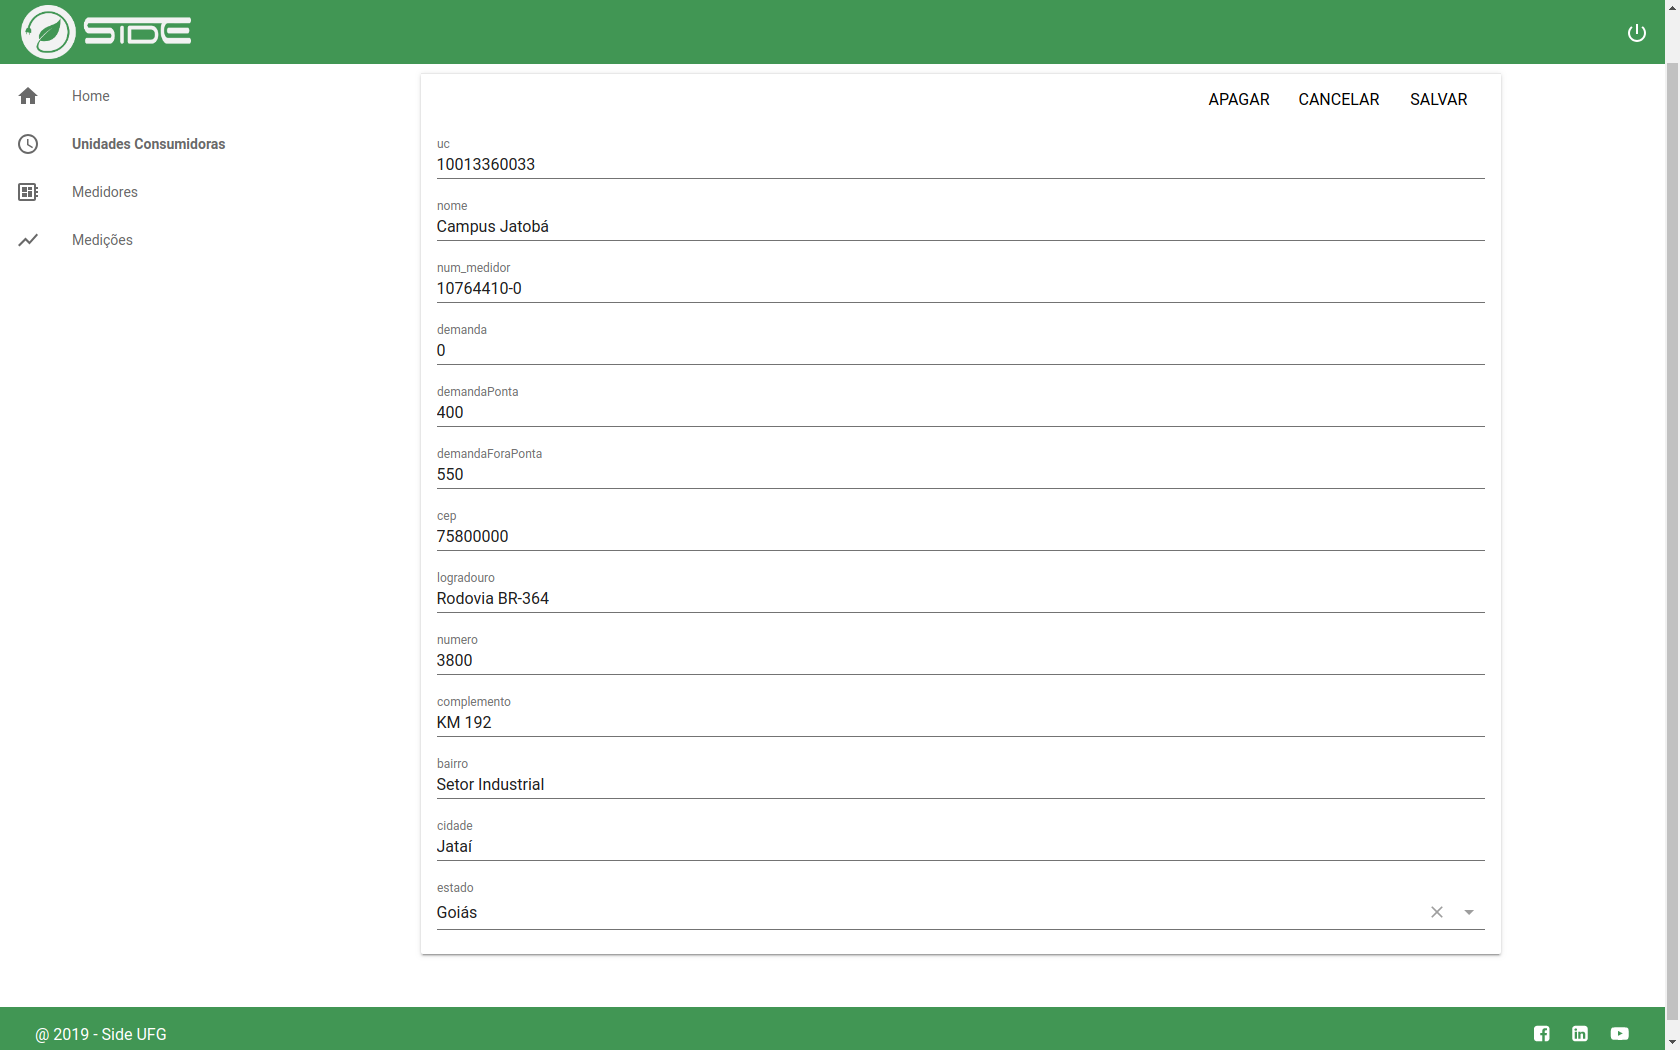
\includegraphics[width=\linewidth]{imagens/side/side-uc-edit.png}
    \caption*{Fonte: Próprio Autor}
    \label{fig:side-uc-edit}
\end{figure}

\subsection{Cadastro de Medidores}

No menu de Medidores podemos visualizar os medidores da Universidade cadastrados na base através do \textit{Side Synchronizer}, descriminados pela denominação do mesmo.

Na listagem de cada medidor, pode-se ver a unidade consumidora associada à ele, o tipo de Medidor, suas coordenadas geográficas, bem como suas datas de início e fim de leitura. Abaixo temos disponível a ação de edição para aquele item. Para a tela de medidores não é permitido cadastras ou remover itens, pois o mesmo só pode ser feito pelo dispositivo mestre da rede \textit{Modbus}.

Na figura \ref{fig:side-medidor-list} temos uma imagem da tela de listagem de medidores do sistema.

\begin{figure}[H]
    \centering
    \caption{Tela de Listagem dos Medidores CCK}
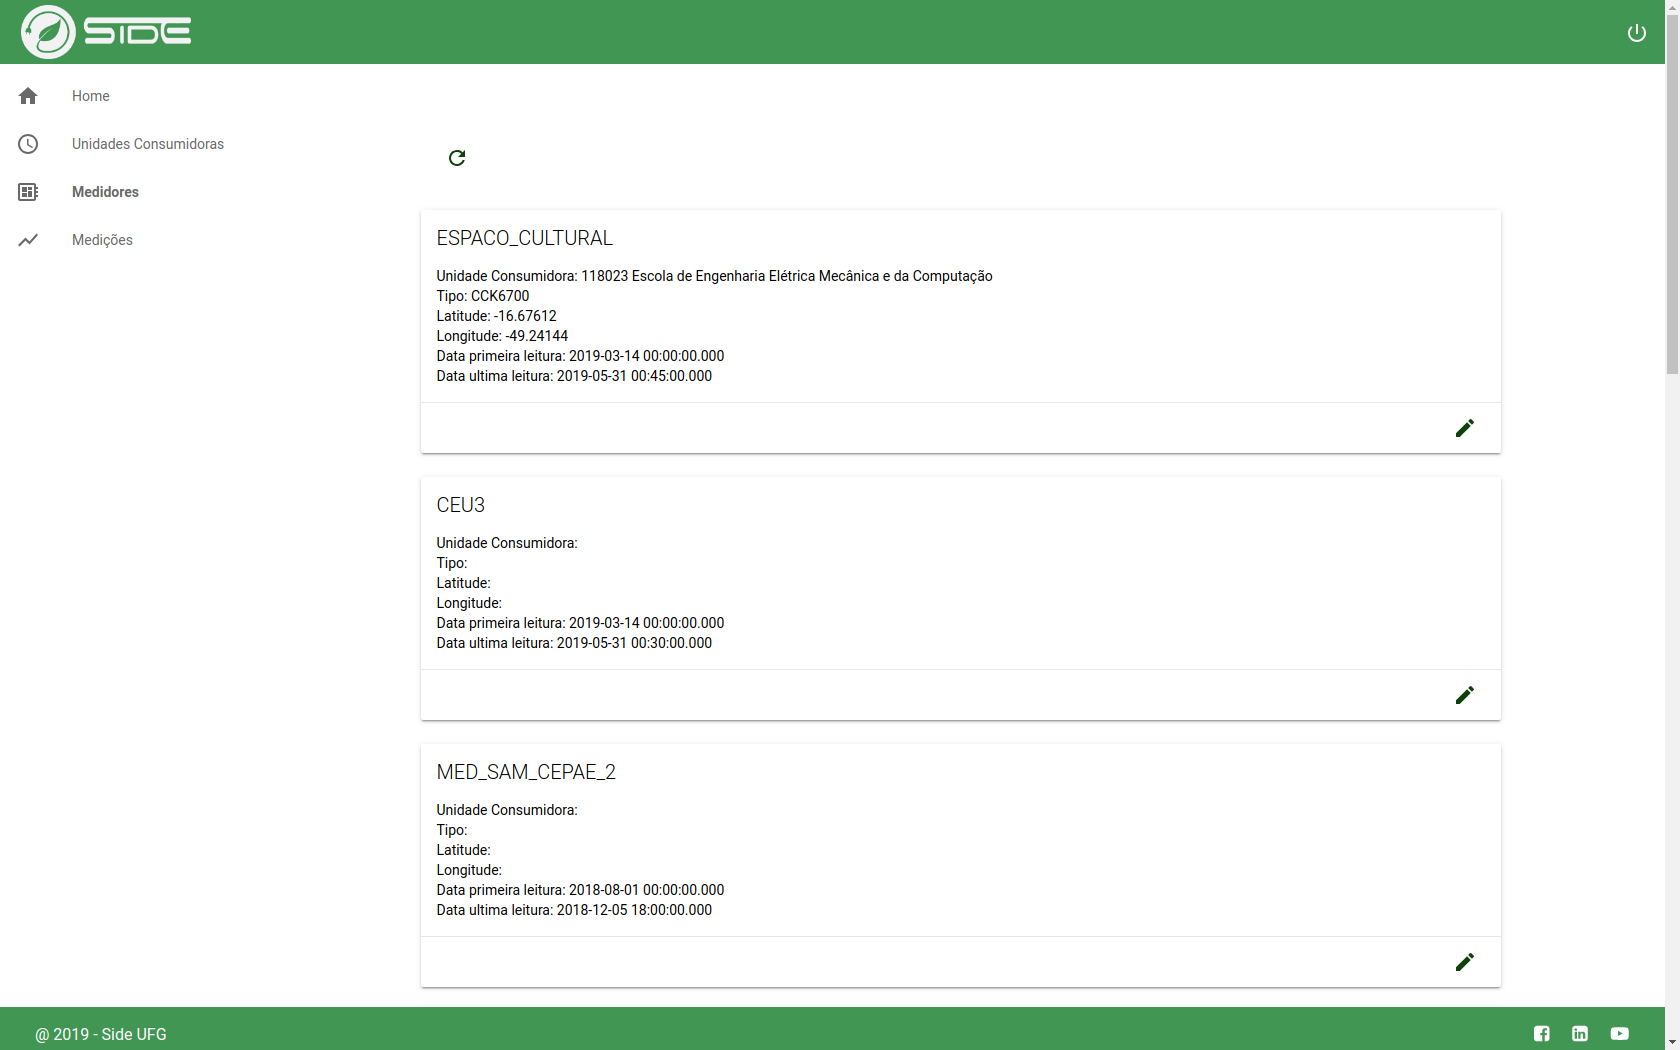
\includegraphics[width=0.75\linewidth]{imagens/side/side-medidor-list.png}
    \caption*{Fonte: Próprio Autor}
    \label{fig:side-medidor-list}
\end{figure}

Ao editar um medidor através do ícone de edição do item, teremos acesso a tela de edição, onde deverão ser preenchidos os dados e após o preenchimento poderão ser salvos. A denominação pode ser alterada pois não interfere na comunicação do \textit{Side Synchronizer} com o mestre da rede \textit{Modbus}, pois a mesma é feita utilizando o id do medidor. Por outro lado não é possível apagar aquele medidor ou criar um novo, essa ação deve ser feita pelo Gerenciador da CCK. 

Na figura \ref{fig:side-medidor-edit} temos uma imagem da tela de edição de medidor:

\begin{figure}[H]
    \centering
    \caption{Tela de Edição dos Medidores}
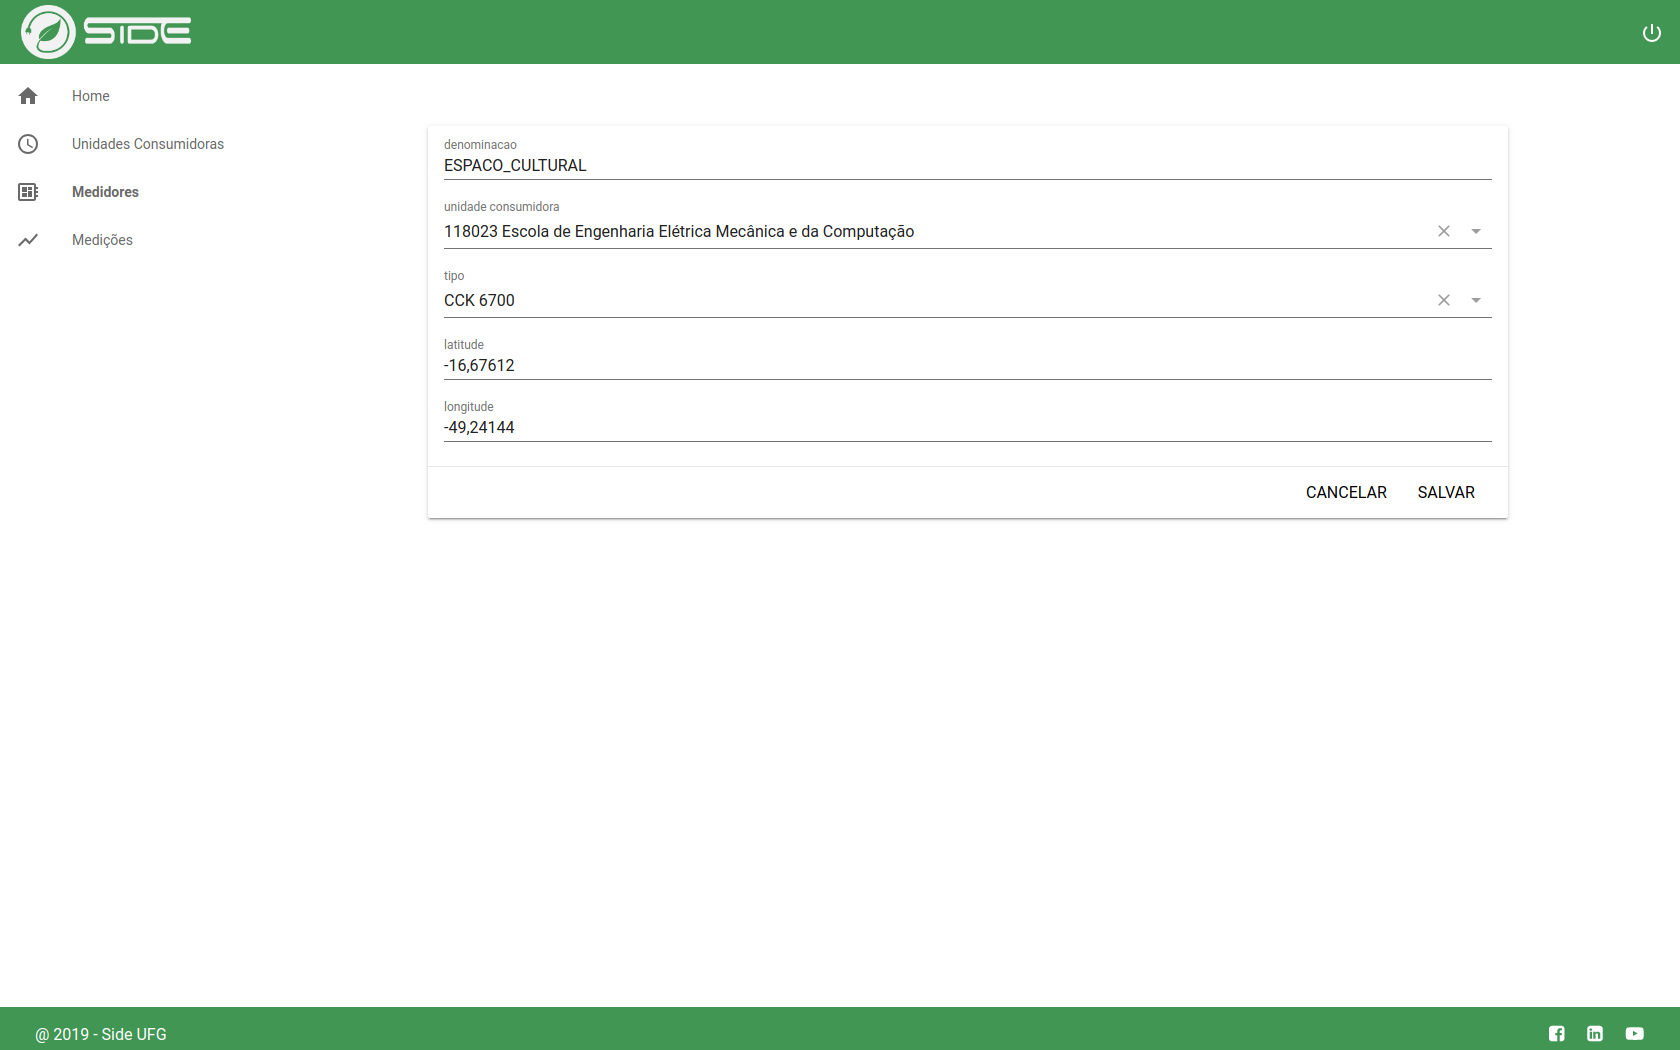
\includegraphics[width=0.75\linewidth]{imagens/side/side-medidor-edit.png}
    \caption*{Fonte: Próprio Autor}
    \label{fig:side-medidor-edit}
\end{figure}


\subsection{Visualização de Medições}

No menu de Medições podemos visualizar o gráfico das medições de um medidor da Universidade cadastrados na base através do \textit{Side Synchronizer}. Além disso as medições podem ser filtradas por data inicial e final.

Ao preencher o filtro da tela selecionando um medidor e suas datas o sistema irá buscar na tabela de medições os resultados limitados pelos parâmetros de busca. Após isso será gerado um gráfico com a curva de potência ativa e reativa distribuídos pelo tempo em um intervalo de 15 minutos.

O gráfico é interativo e permite que o usuário expanda ou comprima os eixos para detalhar melhor as leituras, além disso ao posicionar o ponteiro do mouse sobre um ponto as informações detalhadas daquele ponto serão exibidas.

Na figura \ref{fig:side-medicoes} temos uma imagem da tela de medições com o gráfico gerado através da seleção de um medidor e um intervalo de data.

\begin{figure}[H]
    \centering
    \caption{Tela de Gráfico de Medições}
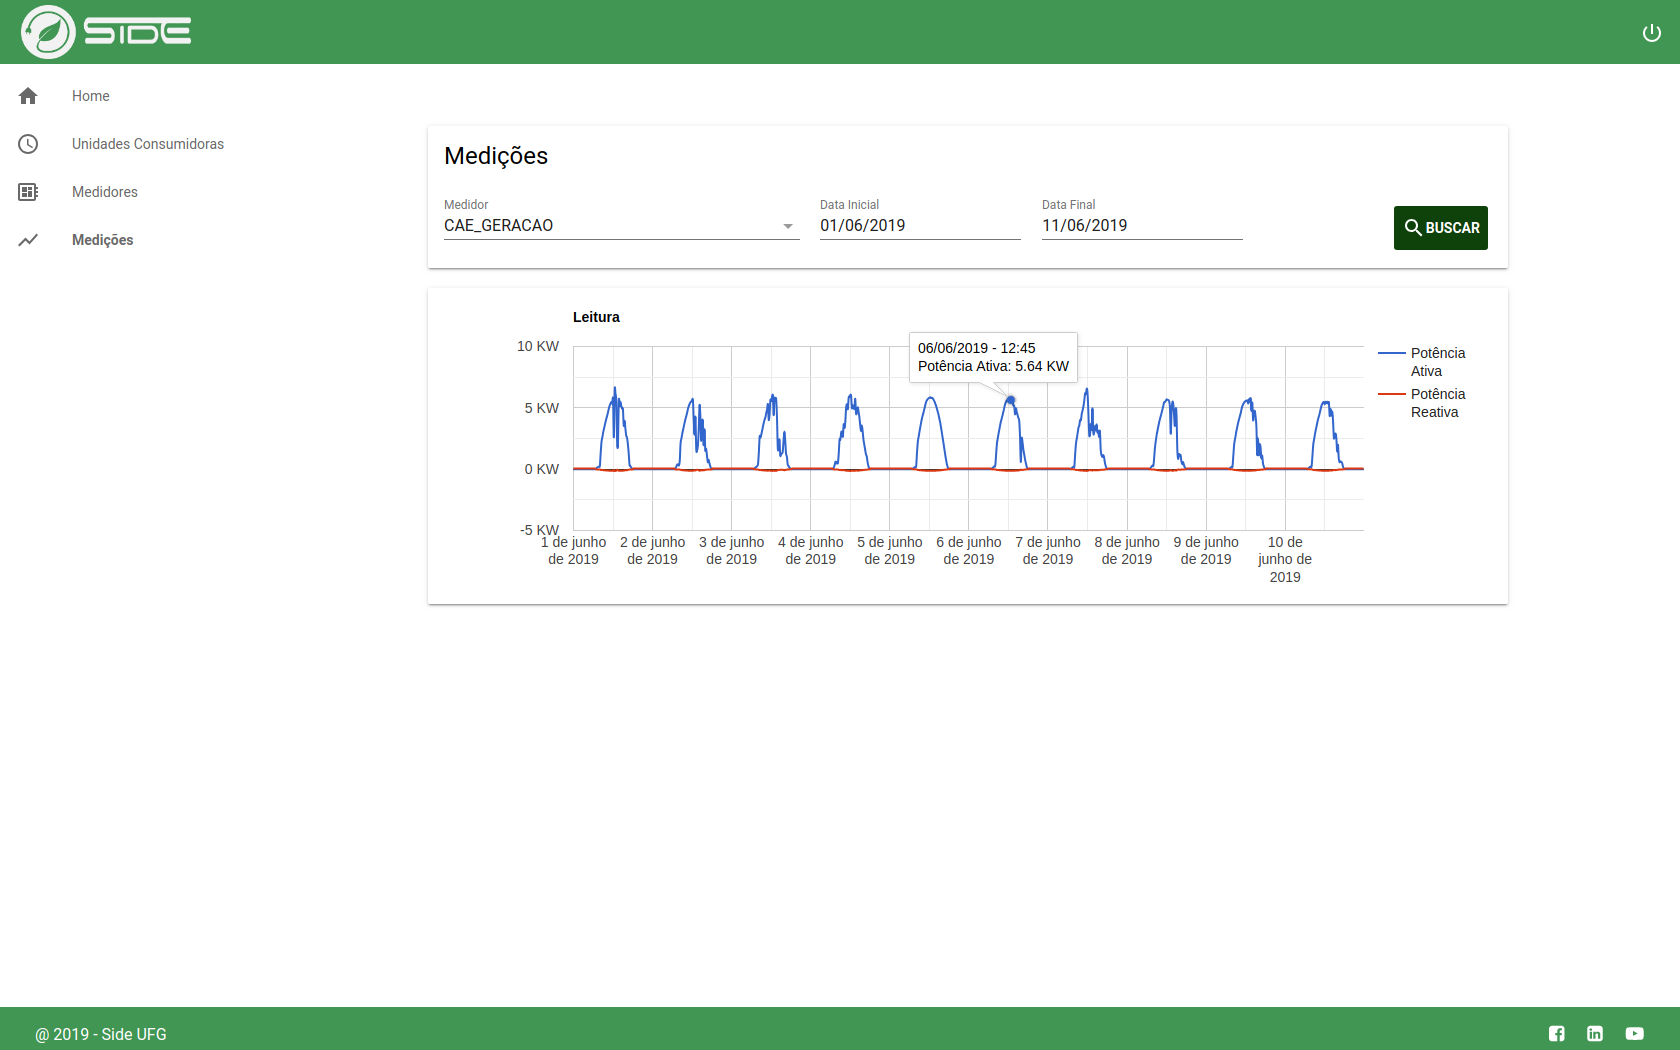
\includegraphics[width=\linewidth]{imagens/side/side-medicoes.png}
    \caption*{Fonte: Próprio Autor}
    \label{fig:side-medicoes}
\end{figure}

% ----------------------------------------------------------
% PARTE
% ----------------------------------------------------------
\part{Resultados}
% ----------------------------------------------------------

\chapter{Obtenção dos Dados dos Sensores}
\label{c:obtencao_dos_dados_dos_sensores}
% ---

% ---
\section{Comunicação}
% ---

\lipsum[21-22]

% ---
% segundo capitulo de Resultados
% ---
\section{Armazenamento}
% ---

\lipsum[23]
\chapter {Obtenção dos Dados das Faturas}
\label{c:obtencao_dos_dados_das_faturas}

Assim como a obtenção dos dados dos sensores, os dados históricos das faturas energéticas são dados importantes para análises financeiras, e o desenvolvimento de um sistema que pudesse extrair esses dados e disponibilizá-los para consulta, tornou o acesso às informações mais fácil.

O trabalho de uma extração de um arquivo PDF, se tornaria algo muito custoso para o estudo caso tivesse que ser feito manualmente, e com o desenvolvimento da aplicação \textit{PdfReader}, esse custo pode ser transferido para se dedicar a análise dos dados em si. 

A possibilidade de extrair esses dados para um arquivo externo do tipo CSV cria o cenário onde se pode entregar esses dados para análise sem dar acesso à todo o restante das informações contidas na base de dados do sistema, focando a análise apenas no histórico de consumo da Universidade. Porém caso seja necessário, devido ao fato de as mesmas informações estarem na base do SIDE, pode-se também fazer uma análise juntamente com os dados das medições, tanto para efeito de auditoria, quanto para efeito de projeções.

Caso futuramente, a concessionária de energia forneça uma API para consulta aos dados das faturas, o sistema pode ser adequado para fazer essa extração diretamente das requisições feitas ao serviço da fornecedora. Além disso esse sistema pode ser adequado à outras cobranças, como fornecimento de água por exemplo.
\chapter {Resultado da Interface do Usuário}
\label{c:resultado_da_interface_do_usuario}

\section{Armazenamento}
% ---
\lipsum[25]
\chapter{Conclusões}
\label{c:conclusoes}

O desenvolvimento do presente projeto possibilitou uma análise de como um sistema feito a partir de um estudo, pode melhorar o estudo do cenário energético da Universidade Federal de Goiás. Além disso também permitiu que fosse analisada a infraestrutura de medição entregue pela Enel à UFG, observando as suas limitações e os seus benefícios para estudos como troca de contrato de demanda, troca de lâmpadas, políticas de redução de consumo, entre outras. Alguns pontos importantes puderam ser obtidos do desenvolvimento desse trabalho:

\begin{itemize}
    \item Multidisciplinaridade: o envolvimento de diversas áreas do conhecimento, como engenharia elétrica, economia, ciências sociais, automação, engenharia de software, entre outras, é de extrema importância para um bom desenvolvimento de um projeto com uma área de atuação tão ampla como este.
    \item Código Livre: o desenvolvimento de um projeto que irá contemplar vários tipos de análises em estudos futuros deve ter o seu código aberto para visualização e contribuição de outros pesquisadores, permitindo que o seu funcionamento não dependa de uma empresa em específico, como é o caso do sistema proprietário da CCK.
    \item Melhoramento da estrutura: um modelo melhor de estrutura física da rede de medição pode ser estudado, de forma a viabilizar uma comunicação mais aberta entre os sensores e os inúmeros meios de interface que poderão existir caso esses dados sejam mais livres. Para o desenvolvimento deste projeto foi necessário inicialmente criar uma maneira de tornar os dados de medição que eram restritos acessíveis livremente, através de um banco de dados, mas se os sensores não fossem de arquitetura fechada, o mesmo poderia ocorrer sem a necessidade de criação desse sistema.
\end{itemize}

Os objetivos iniciais de desenvolver três sistemas responsáveis por obter os dados das medições, obter os dados históricos da concessionária através das faturas, armazenar esses dados, criar uma interface para visualização dos dados de medição, e a implantação de todo esse sistema, disponibilizando-o para uso da instituição, foram atingidos.
\chapter{Trabalhos Futuros}
\label{c:trabalhos_futuros}

\lipsum[31-33]


% ----------------------------------------------------------
% ELEMENTOS PÓS-TEXTUAIS
% ----------------------------------------------------------
\postextual
% ----------------------------------------------------------

% ----------------------------------------------------------
% Referências bibliográficas
% ----------------------------------------------------------
\bibliography{referencias}

% ----------------------------------------------------------
% Glossário
% ----------------------------------------------------------
%
% Consulte o manual da classe abntex2 para orientações sobre o glossário.
%
%\glossary

% ----------------------------------------------------------
% Apêndices
% ----------------------------------------------------------

% ---
% Inicia os apêndices
% ---
\begin{apendicesenv}

% Imprime uma página indicando o início dos apêndices
\partapendices

% ----------------------------------------------------------
\chapter{Desenvolvimento de Sistema para gerenciar e auxiliar na tomada de decisão envolvendo consumo de energia elétrica} \label{a:PFC1}
% ----------------------------------------------------------

Trabalho apresentado pelo aluno {\imprimirautor} na disciplina de PROJETO DE FINAL DE CURSO 1 do Curso de Engenharia de Computação, Goiânia, Julho, 2018.\\

Link para a apresentação no Slideshare: \url{https://www.slideshare.net/ratacheski/apresentao-sideufg}.

% ----------------------------------------------------------
\chapter{Modelagem de Dados do SIDE} \label{a:modelo-dados-side}
% ----------------------------------------------------------

Modelo desenvolvido pelo aluno {\imprimirautor} através do \textit{software DbSchema}, e disponibilizado no servidor Debian de aplicação e banco de dados da Universidade Federal de Goiás, disponível para acesso através da url abaixo.\\

Link para acesso ao modelo de dados:

\url{http://200.137.220.157:8080/sideufg-datamodel/}.

\end{apendicesenv}
% ---


% ----------------------------------------------------------
% Anexos
% ----------------------------------------------------------

% ---
% Inicia os anexos
% ---
\begin{anexosenv}

% Imprime uma página indicando o início dos anexos
\partanexos

% ---
\chapter{Morbi ultrices rutrum lorem.}
% ---
\lipsum[30]

% ---
\chapter{Cras non urna sed feugiat cum sociis natoque penatibus et magnis dis
parturient montes nascetur ridiculus mus}
% ---

\lipsum[31]

% ---
\chapter{Fusce facilisis lacinia dui}
% ---

\lipsum[32]

\end{anexosenv}

%---------------------------------------------------------------------
% INDICE REMISSIVO
%---------------------------------------------------------------------
%\phantompart
\printindex
%---------------------------------------------------------------------

\end{document}
